\subsection{Substitutions}

Let E be an A-algebra. A topology on E is said to be linear if it is invariant under translation and if there exists a fundamental system of neighbourhoods of 0 consisting of ideals of E (Gen.~Top., III, p.~223). The topology on E is then compatible with its A-algebra structure (when A carries the discrete topology). An A-algebra with a linear topology is called a linearly topologized A-algebra.

PROPOSITION 4. --- Let I be a set and E an associative, commutative, unital, linearly topologized separated complete A-algebra.

\begin{enumerate}
\def\labelenumi{(\roman{enumi})}
\tightlist
\item
  Let \(\varphi\) be a continuous homomorphism of A{[}{[}I{]}{]} into E and \(x_{i} = \varphi (\mathbf{X}_{i})\) . Then:
\end{enumerate}

\begin{enumerate}
\def\labelenumi{(\alph{enumi})}
\item
  for all \(i \in \mathbf{I}\) , \(x_{i}^{n}\) tends to 0 as \(n\) tends to \(+\infty\) ;
\item
  if I is infinite, \(x_{i}\) tends to 0 along the filter of complements of finite subsets of I.
\end{enumerate}

\begin{enumerate}
\def\labelenumi{(\roman{enumi})}
\setcounter{enumi}{1}
\tightlist
\item
  Let \(\mathbf{x} = (x_i)_{i\in I}\) be a family of elements of E satisfying \(a\) and \(b\) of (i). Then there exists one and only one unital continuous homomorphism \(\varphi\) of A{[}{[}I{]}{]} into E such that \(\varphi (\mathbf{X}_i) = x_i\) for all \(i\in I\) .
\end{enumerate}

For all \(i \in I\) , \(X_{i}^{n}\) clearly tends to 0 in A{[}{[}I{]}{]} as n tends to \(+\infty\) ; on the other hand when I is infinite, \(X_{i}\) tends to 0 along the filter of complements of finite subsets of I. This proves (i).

Let \((x_{i})_{i\in I}\) be a family of elements of E satisfying conditions \(a)\) and \(b)\) of (i), let \(\psi\) be the homomorphism \(u\mapsto u((x_i)_{i\in I})\) of \(\mathbf{A}[(\mathbf{X}_i)_{i\in I}]\) into E, and let V be a neighbourhood of 0 of E which is an ideal of E. By \(b)\) there exists a finite subset J of I such that \(x_{i}\in \mathbf{V}\) for all \(i\in \mathrm{I - J}\) . Next there exists by \(a)\) an integer \(n\geqslant 0\) such that \(x_{i}^{n}\in \mathbf{V}\) for all \(i\in \mathrm{J}\) . Let \(\beta\) be the element of \(\mathbf{N}^{(I)}\) such that \(\beta_{i} = n - 1\) for \(i\in \mathrm{J}\) and \(\beta_{i} = 0\) for \(i\in \mathrm{I - J}\) . If we define the ideal \(\mathfrak{a}_{\beta}\) of A{[}{[}I{]}{]} as at the beginning of No.~2 (IV, p.~26), then

\[
u \in \mathrm{A} \left[ \left(\mathrm{X} _ {i}\right) _ {i \in I} \right] \cap \mathfrak {a} _ {\beta} \Rightarrow \psi (u) \in \mathrm{V}.
\]

This shows that \(\psi\) is continuous if we equip \(\mathbf{A}[(\mathbf{X}_i)_{i\in I}]\) with the topology induced by that of \(\mathbf{A}[[I]]\) . Since \(\mathbf{E}\) is separated and complete, \(\psi\) extends to a continuous unital homomorphism \(\varphi\) of \(\mathbf{A}[[I]]\) into \(\mathbf{E}\) . We have \(\varphi (\mathbf{X}_i) = \psi (\mathbf{X}_i) = x_i\) for all \(i\in I\) . Finally let \(\varphi^{\prime}\) be a continuous unital homomorphism of \(\mathbf{A}[[I]]\) into \(\mathbf{E}\) such that \(\varphi^{\prime}(\mathbf{X}_{i}) = x_{i}\) . We have \(\varphi^{\prime}(u) = \varphi (u)\) for all \(u\in \mathbf{A}[(\mathbf{X}_i)_{i\in I}]\) , hence \(\varphi^{\prime} = \varphi\) because \(\mathbf{A}[(\mathbf{X}_i)_{i\in I}]\) is dense in \(\mathbf{A}[[I]]\) .

Let us keep the previous notation. If \(u \in \mathbf{A}[[\mathbf{I}]]\) , the image of \(u\) by \(\varphi\) is denoted by \(u(\mathbf{x})\) or \(u((x_i)_{i \in \mathbf{I}})\) (or also \(u(x_1, \ldots, x_n)\) if \(\mathbf{I} = \{1, 2, \ldots, n\}\) ) and is called the element of \(\mathbf{E}\) obtained by substitution of \(x_i\) for \(X_i\) in \(u\) , or the value of \(u\) for the values \(x_i\) of the \(X_i\) or also the value of \(u\) for \(X_i = x_i\) . In particular we have \(u = u((X_i)_{i \in \mathbf{I}})\) .

Let \(E'\) be an associative commutative and unital linearly topologized separated and complete A-algebra. Let \(\lambda\) be a continuous unital homomorphism of E into \(E'\) , and \((x_i)_{i \in I}\) a family of elements of E satisfying conditions \(a)\) and \(b)\) of Prop. 4 (IV, p.~28). The family \((\lambda(x_i))_{i \in I}\) satisfies the same conditions \(a)\) and \(b)\) . For every \(u \in A[[I]]\) we have

\[
\lambda \left(u \left(\left(x _ {i}\right) _ {i \in I}\right)\right) = u \left(\left(\lambda \left(x _ {i}\right)\right) _ {i \in I}\right),\tag{3}
\]

for the mapping \(u \mapsto \lambda(u((x_i)_{i \in I}))\) is a continuous unital homomorphism of \(A[[I]]\) into \(E'\) which transforms \(X_i\) into \(\lambda(x_i)\) for all \(i \in I\) .

If \(J\) and \(K\) are two sets, we denote by \(A_{J,K}\) the set of all families \((g_j)_{j \in J}\) satisfying the following conditions:

\begin{enumerate}
\def\labelenumi{(\roman{enumi})}
\item
  for all \(j \in \mathbf{J}\) , \(g_j\) is an element of \(\mathbf{A}[[\mathbf{K}]]\) whose constant term is nilpotent;
\item
  if \(J\) is infinite, \(g_{j}\) tends to 0 along the filter of complements of finite subsets of \(J\) .
\end{enumerate}

We note that if J is finite, every family of formal power series \((g_{j})_{j\in J}\) without constant term in A{[}{[}K{]}{]} belongs to \(A_{J,K}\) .

Let \((g_j)_{j\in J}\) be in \(\mathbf{A}_{\mathrm{J},\mathbf{K}}\) . By the Cor. of Prop. 3 (IV, p.~28) we have \(\lim_{n\to \infty}g_j^n = 0\) for all \(j\in J\) . Let \(f\in \mathbf{A}[[\mathrm{J}]]\) ; we can substitute \(g_{j}\) for the variable of

index \(j\) in \(f\) and obtain a formal power series \(f((g_j)_{j \in J})\) belonging to A{[}{[}K{]}{]}. Moreover, the mapping \(f \mapsto f((g_j)_{j \in J})\) is a continuous homomorphism of A-algebras A{[}{[}J{]}{]} into A{[}{[}K{]}{]}.

In particular if \(J = \{1, \ldots, p\}\) and \(f \in A[[X_1, \ldots, X_p]]\) , we can substitute for each \(X_j\) a formal power series \(g_j \in A[[K]]\) without constant term; the result of this substitution is written \(f(g_1, \ldots, g_p)\) .

Let \(\mathbf{x} = (x_k)_{k\in K}\) be a family of elements of E satisfying conditions \(a\) and \(b\) ) of Prop. 4 (IV, p.~28). Let us apply (3), taking for \(\lambda\) the homomorphism \(u\mapsto u(\mathbf{x})\) of A{[}{[}K{]}{]} into E; we obtain

\[
f \left(\left(g _ {j}\right) _ {j \in J}\right) (\mathbf {x}) = f \left(\left(g _ {j} (\mathbf {x})\right) _ {j \in J}\right).\tag{4}
\]

Let \(\mathbf{f} = (f_i)_{i\in I}\in (\mathbf{A}[[J]])^I\) and \(g = (g_j)_{j\in J}\in \mathbf{A}_{J,K}\) . We denote by \(\mathbf{f}(\mathbf{g})\) or \(\mathbf{f}\circ \mathbf{g}\) the element \((f_{i}((g_{j})_{j\in J}))_{i\in I}\) of \((\mathbf{A}[[K]])^I\) . If \(\mathbf{f}\in \mathbf{A}_{I,J}\) , we have \(\mathbf{f}\circ \mathbf{g}\in \mathbf{A}_{I,K}\) because the mapping \(f\mapsto f((g_j)_{j\in J})\) of \(\mathbf{A}[[I]]\) into \(\mathbf{A}[[K]]\) is continuous.

Let \(\mathbf{f} \in (\mathbf{A}[[J]])^{\mathrm{I}}\) , \(\mathbf{g} \in \mathbf{A}_{\mathrm{J},\mathrm{K}}\) , \(\mathbf{h} \in \mathbf{A}_{\mathrm{K},\mathrm{L}}\) . Then \(\mathbf{g} \circ \mathbf{h} \in \mathbf{A}_{\mathrm{J},\mathrm{L}}\) and by (4), we have

\[
(\mathbf {f} \circ \mathbf {g}) \circ \mathbf {h} = \mathbf {f} \circ (\mathbf {g} \circ \mathbf {h}).\tag{5}
\]

\subsection{Invertible formal power series}

PROPOSITION 5. --- In the ring A{[}{[}T{]}{]} of formal power series in one indeterminate the polynomial 1 - T is invertible, and we have \((1 - \mathrm{T})^{-1} = \sum_{n=0}^{\infty} \mathrm{T}^{n}\) .

For

\[
(1 - \mathrm{T}) \left(\sum_ {n = 0} ^ {\infty} \mathrm{T} ^ {n}\right) = \sum_ {n = 0} ^ {\infty} \mathrm{T} ^ {n} - \sum_ {n = 0} ^ {\infty} \mathrm{T} ^ {n + 1} = 1.
\]

PROPOSITION 6. --- Let \(u \in \mathbf{A}[[\mathbf{I}]]\) ; then for \(u\) to be invertible in \(\mathbf{A}[[\mathbf{T}]]\) it is necessary and sufficient that its constant term should be invertible in \(\mathbf{A}\) .

Suppose that there exists \(v \in A[[I]]\) such that \(uv = 1\) . Let \(\alpha, \beta\) be the constant terms of \(u\) and \(v\) , then \(\alpha\beta = 1\) , so \(\alpha\) is invertible.

Conversely, suppose that the constant term \(\alpha\) of \(u\) is invertible. Then there exists a formal power series \(t \in \mathbf{A}[[\mathrm{I}]]\) such that \(u = \alpha(1 - t)\) and \(\omega(t) > 0\) . Now there is a ring homomorphism \(\varphi: \mathbf{A}[[\mathrm{T}]] \to \mathbf{A}[[\mathrm{I}]]\) such that \(\varphi(\mathrm{T}) = t\) , and \(1 - \mathrm{T}\) is invertible in \(\mathbf{A}[[\mathrm{T}]]\) (Prop. 5); consequently \(1 - t\) is invertible in \(\mathbf{A}[[\mathrm{I}]]\) , and hence so is \(u\) .

Remark. --- Let M be the set of all formal power series with constant term 1. By Prop. 6, M is a commutative group under multiplication; the multiplicative group of A{[}{[}I{]}{]} is thus the direct product of M and the multiplicative group of A. We shall equip M with the topology induced from that of A{[}{[}I{]}{]}. For each \(\beta \in \mathbf{N}^{(I)}\) we have in IV, p.~26 defined the ideal \(a_{\beta}\) of A{[}{[}I{]}{]}; then \(1 + a_{\beta}\) is a subgroup of M and the family \((1 + a_{\beta})\) is a fundamental system of neighbourhoods of 1 in M. Since the multiplication in M is continuous, we see that M is a topological group (Gen.~Top., III, p.~223); in other words, the mapping \(f \mapsto f^{-1}\) is continuous in M.

Let K be a commutative field and \(\mathfrak{D}\) the subring of the field of rational fractions \(\mathrm{K}((\mathbf{X}_i)_{i\in I})\) formed of rational fractions in which the element 0 of \(\mathbf{K}^I\) is substitutable. If \(f\in \mathfrak{D}\) , we have \(f = \frac{u}{v}\) , where \(u\) and \(v\) are polynomials such that the constant term of \(v\) is \(\neq 0\) , hence \(v\) is invertible in \(\mathbf{K}[[\mathrm{I}]]\) . We can verify at once that the element \(uv^{-1}\) of \(\mathbf{K}[[\mathrm{I}]]\) depends only on \(f\) ; we say that the formal power series \(uv^{-1}\) is the expansion at the origin of the rational fraction \(\frac{u}{v}\) . The mapping \(f\mapsto uv^{-1}\) is an injective homomorphism of \(\mathfrak{D}\) into \(\mathbf{K}[[\mathrm{I}]]\) ; we shall often identify \(\mathfrak{D}\) with its image under this mapping.

\subsection{Taylor's formula for formal power series}

Let \(\mathbf{X} = (\mathbf{X}_i)_{i\in I}\) and \(\mathbf{Y} = (\mathbf{Y}_i)_{i\in I}\) be two families of indeterminates relative to the same index set I. We denote by \(\mathbf{X} + \mathbf{Y}\) the family \((\mathbf{X}_i + \mathbf{Y}_i)_{i\in I}\) of formal power series in \(\mathbf{A}[[\mathbf{X},\mathbf{Y}]]\) . It is clear that we can substitute \(\mathbf{X}_i + \mathbf{Y}_i\) for \(\mathbf{X}_i\) in a formal power series \(u\in \mathbf{A}[[\mathbf{X}]]\) , the result being written \(u(\mathbf{X} + \mathbf{Y})\) . For each \(\nu \in \mathbf{N}^{(I)}\) we denote by \(\Delta^{\nu}u\) the coefficient of \(\mathbf{Y}^{\nu}\) in the formal power series \(u(\mathbf{X} + \mathbf{Y})\) considered as belonging to \(\mathbf{A}[[\mathbf{X}]][[\mathbf{Y}]]\) (III, p.~456). In other words, we have

\[
u (\mathbf {X} + \mathbf {Y}) = \sum_ {\nu} \Delta^ {\nu} u (\mathbf {X}) \cdot \mathbf {Y} ^ {\nu} \quad (u \in \mathrm{A} [ [ \mathbf {X} ] ]).\tag{6}
\]

Substituting (0, X) for (X, Y) we obtain

\[
u (\mathbf {X}) = \sum_ {\nu} \Delta^ {\nu} u (0) \cdot \mathbf {X} ^ {\nu};\tag{7}
\]

In other words, the constant term of \(\Delta^{\nu}u\) is the coefficient of \(\mathbf{X}^{\nu}\) in \(u\) . Since the mapping \(u \mapsto u(\mathbf{X} + \mathbf{Y})\) of \(\mathbf{A}[[\mathbf{X}]]\) into \(\mathbf{A}[[\mathbf{X}, \mathbf{Y}]]\) is continuous, the mappings \(u \mapsto \Delta^{\nu}u\) of \(\mathbf{A}[[\mathbf{X}]]\) into itself are again continuous.

As in the case of polynomials (IV, p.~7) we can prove the formulae

\begin{enumerate}
\def\labelenumi{(\arabic{enumi})}
\setcounter{enumi}{7}
\tightlist
\item
\end{enumerate}

\[
\Delta^ {\sigma} (u v) = \sum_ {\nu + \rho = \sigma} \Delta^ {\nu} (u) \Delta^ {\rho} (v),
\]

\[
\Delta^ {\rho} \Delta^ {\sigma} u = \frac {(\rho + \sigma) !}{\rho ! \sigma !} \Delta^ {\rho + \sigma} u.\tag{9}
\]

The binomial formula (I, p.~99, Cor. 2) gives the following value for \(\Delta^{\nu}u\) when \(u = \sum_{\lambda} \alpha_{\lambda} X^{\lambda}\)

\[
\Delta^ {\nu} u = \sum_ {\lambda} \alpha_ {\lambda + \nu} \frac {(\lambda + \nu) !}{\lambda ! \nu !} X ^ {\lambda}.\tag{10}
\]

Consider in particular the case \(\nu = \varepsilon_{i}\) , that is \(\nu_{i} = 1\) , \(\nu_{j} = 0\) for \(j \neq i\) . We shall put \(D_{i}u = \Delta^{\varepsilon_{i}}u\) ; put differently, \(D_{i}u\) is the coefficient of \(Y_{i}\) in \(u(\mathbf{X} + \mathbf{Y})\) . By (10) we thus have

\[
\mathrm{D} _ {i} u = \sum_ {\lambda} (\lambda_ {i} + 1) \alpha_ {\lambda + \varepsilon_ {i}} X ^ {\lambda};\tag{11}
\]

in particular we have \(\mathbf{D}_{i}(\mathbf{X}_{i})=1\) and \(\mathbf{D}_{i}(\mathbf{X}_{j})=0\) for \(j\neq i\) . The formula (8) shows that \(D_{i}\) is a derivation of A{[}{[}X{]}{]}, and from (9) we deduce the relation

\[
\mathbf {D} ^ {\nu} \boldsymbol {u} = \nu ! \Delta^ {\nu} \boldsymbol {u}\tag{12}
\]

as in the case of polynomials (IV, p.~8) (we have put \(\mathbf{D}^{\nu} = \prod_{i\in I}\mathbf{D}_{i}^{\nu_{i}}\) for \(\nu = (\nu_{i})_{i\in I}\) in \(\mathbf{N}^{(I)}\) ). When \(\mathbf{A}\) is a \(\mathbf{Q}\) -algebra, the formulae (6), (7) and (12) imply the « Taylor formulae »:

\begin{enumerate}
\def\labelenumi{(\arabic{enumi})}
\setcounter{enumi}{12}
\tightlist
\item
\end{enumerate}

\[
u (\mathbf {X} + \mathbf {Y}) = \sum_ {\nu} \frac {1}{\nu !} D ^ {\nu} u (\mathbf {X}). \mathbf {Y} ^ {\nu},
\]

\[
u (\mathbf {X}) = \sum_ {\nu} \frac {1}{\nu !} D ^ {\nu} u (0) \cdot X ^ {\nu}.\tag{14}
\]

Remarks. --- 1) We often say that \(D_i u\) is the partial derivative of \(u\) with respect to \(X_i\) ; we also use the notation \(D_{X_i} u, \frac{\partial u}{\partial X_i}\) and \(u_{X_i}'\) . For a single indeterminate \(X\) the unique partial derivative \(Du\) (also written \(\frac{du}{dX}\) or \(u'\) ) is called the derivative of \(u\) .

\begin{enumerate}
\def\labelenumi{\arabic{enumi})}
\setcounter{enumi}{1}
\item
  The formula (9) shows that the endomorphisms \(\Delta^{\rho}\) of the A-module \(\mathbf{A}[[\mathbf{X}]]\) commute pairwise. Hence the same holds of the endomorphisms \(D_i\) .
\item
  If \(u \in \mathbf{A}[(\mathbf{X}_i)_{i \in I}]\) is a polynomial, the polynomials \(\Delta^{\rho} u\) and \(D_i u\) defined in IV, p.~6 and 7 coincide with the formal power series denoted by the same symbols.
\end{enumerate}

\subsection{Derivations in the algebra of formal power series}

Let I be a set, E an associative, commutative and unital linearly topologized, separated and complete A-algebra, and \(\mathbf{x} = (x_{i})_{i \in I}\) a family of elements of E satisfying conditions a) and b) of Prop. 4 (IV, p.~28). Let \(\varphi\) be the continuous homomorphism \(u \mapsto u(x)\) of A{[}{[}I{]}{]} into E; it equips E with an A{[}{[}I{]}{]}-module structure. By III, p.~552, an A-derivation D of A{[}{[}I{]}{]} into the A{[}{[}I{]}{]}-module E is thus an A-linear mapping D: A{[}{[}I{]}{]} → E satisfying the relation

\[
\mathrm{D} (u v) = u (\mathbf {x}) \cdot \mathrm{D} (v) + \mathrm{D} (u) \cdot v (\mathbf {x})\tag{15}
\]

for u, v in A{[}{[}I{]}{]}.

PROPOSITION 7. --- Let \((y_{i})_{i\in I}\) be a family of elements of E. When I is infinite, we assume that \(y_{i}\) tends to 0 along the filter of complements of finite subsets of I. There exists then a unique continuous A-derivation D of A{[}{[}I{]}{]} into the A{[}{[}I{]}{]}-module E such that \(\mathrm{D}(\mathbf{X}_{i})=y_{i}\) for all \(i\in I\) . We have

\[
\mathrm{D} (u) = \sum_ {i \in I} (\mathrm{D} _ {i} u) (\mathbf {x}) \cdot y _ {i} \quad (u \in \mathrm{A} [ [ I ] ])  .\tag{16}
\]

Since 0 admits in E a fundamental system of neighbourhoods consisting of ideals, the family \(((\mathrm{D}_i u)(\mathbf{x}) \cdot y_i)_{i \in I}\) is summable in E for all \(u \in A[[I]]\) (Gen.~Top., III, p.~263, Cor. 2). Formula (16) thus defines an A-linear mapping \(\mathbf{D}: A[[I]] \to E\) . We leave the reader to verify that D is a continuous derivation. Let \(\mathbf{D}_1\) be a continuous A-derivation of A{[}{[}I{]}{]} into E, such that \(\mathbf{D}_1(\mathbf{X}_i) = y_i\) for all \(i \in I\) . The kernel of the continuous derivation \(\mathbf{D} - \mathbf{D}_1\) is a closed subalgebra B of A{[}{[}I{]}{]} containing 1 and the indeterminates \(X_{i}\) . Since the polynomial algebra \(\mathbf{A}[(\mathbf{X}_{i})_{i\in I}]\) is dense in A{[}{[}I{]}{]}, we have \(B = A[[I]]\) and so \(D_{1} = D\) .

COROLLARY 1. --- Let \(\Delta\) be a continuous derivation of the A-algebra E. For every formal power series \(u \in \mathbf{A}[[\mathrm{I}]]\) the family \(((\mathrm{D}_i u)(\mathbf{x}) \cdot \Delta x_i)_{i \in I}\) is summable and we have

\[
\Delta (u (\mathbf {x})) = \sum_ {i \in I} \left(\mathrm{D} _ {i} u\right) (\mathbf {x}) \cdot \Delta x _ {i}.\tag{17}
\]

This follows from Prop. 7 because the mapping \(u \mapsto \Delta(u(\mathbf{x}))\) is a continuous derivation of \(\mathbf{A}[[\mathbf{I}]]\) into the \(\mathbf{A}[[\mathbf{I}]]\) -module \(\mathbf{E}\) .

COROLLARY 2. --- The derivation \(D_{i}\) is the unique continuous derivation of the A-algebra A{[}{[}I{]}{]} such that

\[
\mathrm{D} _ {i} (\mathrm{X} _ {i}) = 1, \quad \mathrm{D} _ {i} (\mathrm{X} _ {j}) = 0 \quad f o r \quad j \neq i.\tag{18}
\]

This follows from Cor. 1.

COROLLARY 3. --- Let \(f \in \mathbf{A}[[\mathbf{X}_1, \ldots, \mathbf{X}_p]]\) and \(g_i \in \mathbf{A}[[\mathbf{Y}_1, \ldots, \mathbf{Y}_q]]\) for \(1 \leqslant i \leqslant p\) . Suppose that for \(1 \leqslant i \leqslant p\) the constant term of \(g_i\) is zero, and put \(h = f(g_1, \ldots, g_p)\) . Then for \(1 \leqslant j \leqslant q\) we have

\[
\frac {\partial h}{\partial \mathbf {Y} _ {j}} = \sum_ {i = 1} ^ {p} \mathrm{D} _ {i} f (g _ {1}, \dots , g _ {p}) \cdot \frac {\partial g _ {i}}{\partial \mathbf {Y} _ {j}}.\tag{19}
\]

This is the special case \(\mathbf{E} = \mathbf{A}[[\mathbf{Y}_1,\dots ,\mathbf{Y}_q]]\) , \(x_{i} = q_{i}\) and \(\Delta = \partial /\partial \mathbf{Y}_j\) of Cor. 1.

PROPOSITION 8. --- Let \(\mathbf{X} = (\mathbf{X}_i)_{i\in I}\) be a finite family of indeterminates.

\begin{enumerate}
\def\labelenumi{(\roman{enumi})}
\item
  Every derivation of the ring of formal power series A{[}{[}X{]}{]} is continuous.
\item
  Every derivation of the polynomial ring A{[}X{]} into the ring of formal power series A{[}{[}X{]}{]} extends in a unique fashion to a derivation of the ring A{[}{[}X{]}{]}.
\item
  The family \((\mathbf{D}_i)_{i\in I}\) is a basis of the \(\mathbf{A}[[\mathbf{X}]]\) -module of \(\mathbf{A}\) -derivations of \(\mathbf{A}[[\mathbf{X}]]\) into itself.
\end{enumerate}

Let \(\mathfrak{b}_n\) be the set of all formal power series of order \(\geqslant n\) . It is clear that \(\mathfrak{b}_n\) is an ideal in the ring \(A[[X]]\) , generated by the monomials of degree \(n\) . Hence \(\mathfrak{b}_n\) consists of finite sums of products of \(n\) formal power series without constant terms; if \(D\) is a derivation of \(A[[X]]\) , we have

\[
\mathrm{D} (f _ {1} \dots f _ {n}) = \sum_ {i = 1} ^ {n} f _ {1} \dots f _ {i - 1} \mathrm{D} (f _ {i}) f _ {i + 1} \dots f _ {n},
\]

whence it follows at once that \(\mathbf{Db}_{n} \subset \mathbf{b}_{n-1}\) for \(n \geqslant 1\) . Since the sequence \((\mathfrak{b}_n)_{n \geqslant 0}\) is a fundamental system of neighbourhoods of 0 in A{[}{[}X{]}{]} (IV, p.~26 remark), D is continuous and (i) is proved.

Let \(\Delta\) be a derivation of A{[}X{]} into A{[}{[}X{]}{]}. Arguing as before, we can show that \(\Delta(h)\) belongs to \(\mathfrak{b}_{n-1}\) for every homogeneous polynomial \(h\) of degree \(n \geqslant 1\) . Now let \(u \in \mathbf{A}[[\mathbf{X}]]\) and let \(u_n\) be the homogeneous component of degree \(n\) of \(u\) . Since \(\Delta(u_n) \in \mathfrak{b}_{n-1}\) for \(n \geqslant 1\) , the family \((\Delta(u_n))_{n \geqslant 0}\) is summable in A{[}{[}X{]}{]} and we can define a derivation D of A{[}{[}X{]}{]} into itself by

\[
\mathrm{D} (u) = \sum_ {n \geqslant 0} \Delta \left(u _ {n}\right).
\]

We have \(D(\mathfrak{b}_n) \subset \mathfrak{b}_{n-1}\) , hence \(D\) is a continuous endomorphism of the additive group of \(A[[X]]\) . The mapping \(\Phi: (u, v) \mapsto D(uv) - uD(v) - D(u)v\) of \(A[[X]] \times A[[X]]\) into \(A[[X]]\) is continuous and zero on \(A[X] \times A[X]\) . Since \(A[X]\) is dense in \(A[[X]]\) , we have \(\Phi = 0\) ; in other words, \(D\) is a derivation of \(A[[X]]\) into itself, extending \(\Delta\) .

Finally, A{[}X{]} is dense in A{[}{[}X{]}{]} and every derivation of A{[}{[}X{]}{]} is continuous by (i); hence there exists a unique extension of \(\Delta\) to a derivation of A{[}{[}X{]}{]}. This proves (ii).

It remains to prove (iii). Formula (18) (IV, p.~33) shows that the family \((\mathbf{D}_i)_{i\in I}\) is linearly independent over \(\mathbf{A}[[\mathbf{X}]]\) , and formula (16) (IV, p.~32), applied in the case \(\mathbf{E} = \mathbf{A}[[\mathbf{X}]]\) , shows that every A-derivation is a linear combination of the \(\mathbf{D}_i\) with coefficients in \(\mathbf{A}[[\mathbf{X}]]\) .

PROPOSITION 9. --- Let \((u_{\lambda})_{\lambda \in L}\) be a summable family of elements of A{[}{[}I{]}{]} without constant term and D a continuous derivation of the A-algebra A{[}{[}I{]}{]}. If \(f = \prod_{\lambda \in L} (1 + u_{\lambda})\) (IV, p.~27, Prop. 2), then the family \((D u_{\lambda} / (1 + u_{\lambda}))_{\lambda \in L}\) is

summable and we have

\[
\mathrm{D} (f) / f = \sum_ {\lambda \in L} \mathrm{D} (u _ {\lambda}) / (1 + u _ {\lambda}).\tag{20}
\]

If \(g\) and \(h\) are two invertible elements of \(\mathbf{A}[[\mathbf{I}]]\) , then

\[
\mathrm{D} (g h) = h. \mathrm{D} g + g. \mathrm{D} h
\]

whence on division by gh,

\[
\mathrm{D} (g h) / g h = \mathrm{D} (g) / g + \mathrm{D} (h) / h.\tag{21}
\]

For every finite subset M of L put \(f_{M} = \prod_{\lambda \in M} (1 + u_{\lambda})\) . From (21) we deduce by induction on Card M the relation

\[
\mathrm{D} \left(f _ {\mathrm{M}}\right) / f _ {\mathrm{M}} = \sum_ {\lambda \in \mathrm{M}} \mathrm{D} \left(u _ {\lambda}\right) / \left(1 + u _ {\lambda}\right).\tag{22}
\]

This proves Prop. 9 when L is finite. Now suppose that L is infinite and write F for the filtered ordered set of finite subsets of L. We have \(\lim_{\mathfrak{F}} f_{M} = f\) , and hence (IV, p.~30 remark)

\[
\mathrm{D} (f) / f = \lim _ {\mathfrak {F}} \mathrm{D} (f _ {\mathrm{M}}) / f _ {\mathrm{M}}.
\]

Now Prop. 9 follows by passage to the limit in (22).

\subsection{The solution of equations in a formal power series ring}

Lemma 2. --- Let \((g_i)_{i \in I}\) be a family of elements of order \(\geqslant 2\) in A{[}{[}I{]}{]}. When I is infinite, assume that \(g_i\) tends to 0 along the filter of complements of finite subsets of I. There exists one and only one automorphism T of the topological A-algebra A{[}{[}I{]}{]} such that T(X \(_i\) ) = X \(_i\) + g \(_i\) for all i ∈ I. Further,

\[
\omega (\mathrm{T} (u) - u) \geqslant \omega (u) + 1\tag{23}
\]

for each \(u \in \mathbf{A}[[\mathrm{I}]]\) .

The series \(f_{i} = \mathbf{X}_{i} + g_{i}\) has no constant term and when I is infinite, \(f_{i}\) tends to 0 along the filter of complements of finite subsets of I. Therefore (IV, p.~28, Prop. 4) there exists precisely one continuous endomorphism T of the A-algebra A{[}{[}I{]}{]} such that \(\mathrm{T}(\mathbf{X}_i) = f_i\) for all \(i \in I\) . For each \(\nu \in \mathbf{N}^{(I)}\) we put

\[
v _ {\nu} = \mathrm{T} \left(\mathbf {X} ^ {\nu}\right) - \mathbf {X} ^ {\nu} = \prod_ {i \in I} \left(\mathbf {X} _ {i} + g _ {i}\right) ^ {\nu (i)} - \prod_ {i \in I} \mathbf {X} _ {i} ^ {\nu (i)};
\]

the relations \(\omega(g_i) \geqslant 2\) imply \(\omega(v_\nu) \geqslant |\nu| + 1\) , and the relation (23) follows at once from this.

Let us show that T is injective. Given \(u \in A[[I]]\) such that \(T(u) = 0\) , by (23) we have \(\omega(u) \geqslant \omega(u) + 1\) , which is impossible if \(u \neq 0\) because \(\omega(u)\) would then be a positive integer.

For every formal series \(v\) in \(A[[I]]\) we denote by \(H_n(v)\) its homogeneous component of degree \(n\) . Let us put \(S_0(v) = H_0(v)\) and define the continuous mappings \(S_n: A[[I]] \to A[[I]]\) by the recursion equations

\[
\mathrm{S} _ {n} (v) = \mathrm{H} _ {n} \left(v - \mathrm{T} \left(\sum_ {k = 0} ^ {n - 1} \mathrm{S} _ {k} (v)\right)\right) \quad \text { for } \quad n \geqslant 1.\tag{24}
\]

Put \(S(v) = \sum_{n \geqslant 0} S_n(v)\) ; if \(\nu \in \mathbf{N}^{(I)}\) and \(n = |\nu|\) , then the coefficient \(S^{\nu}(v)\) of

\(X^{\nu}\) in \(S(v)\) is equal to that of \(X^{\nu}\) in \(S_{n}(v)\) ; since \(S_{n}\) is a continuous mapping, the mapping \(S^{\nu}: A[[I]] \to A\) is continuous. Hence, by the definition of the product topology on \(A[[I]] = A^{N^{(I)}}\) , the mapping \(S: A[[I]] \to A[[I]]\) is continuous.

We shall prove the relation \(\mathrm{T}(\mathrm{S}(v)) = v\) for all \(v \in A[[I]]\) which will complete the proof of the lemma. Let \(v \in A[[I]]\) , \(u_n = S_n(v)\) and \(u = S(v)\) . Let n be a positive integer such that

\[
\omega (v - \mathrm{T} (u)) \geqslant n.\tag{$(25)_{n}$}
\]

We have \(\omega(u - (u_{0} + \cdots + u_{n-1})) \geqslant n\) , whence

\[
\omega (\mathrm{T} (u) - \mathrm{T} (u _ {0} + \dots + u _ {n - 1}) - u _ {n}) \geqslant n + 1\tag{26}
\]

by (23). Now the recursion equation (24) shows that

\[
u _ {n} = \mathrm{H} _ {n} (v - \mathrm{T} (u _ {0} + \dots + u _ {n - 1}))\tag{27}
\]

By (26) the formal power series \(v - \mathrm{T}(u)\) and \(v - \mathrm{T}(u_{0} + \cdots + u_{n-1}) - u_{n}\) have the same homogeneous component of degree n, and this component is zero, by (27). We thus have \(\omega(v - \mathrm{T}(u)) \geqslant n + 1\) , that is \((25)_{n}\) implies \((25)_{n+1}\) . Since \((25)_{0}\) clearly holds, we thus have \(\omega(v - \mathrm{T}(u)) \geqslant n\) for every integer \(n \geqslant 0\) , whence \(v = \mathrm{T}(u) = \mathrm{T}(\mathrm{S}(v))\) , as was to be proved.

For the rest of this No.~we shall, for any set I, denote by A \{I\} the set of families \((f_i)_{i\in I}\) satisfying the following conditions:

\begin{enumerate}
\def\labelenumi{(\roman{enumi})}
\item
  for each \(i \in I\) , \(f_i\) is an element of A{[}{[}I{]}{]} without constant term;
\item
  if I is infinite, \(f_{i}\) tends to 0 along the filter of complements of finite subsets of I.
\end{enumerate}

The set A\{I\} is a monoid for the composition law \((\mathbf{f},\mathbf{g})\mapsto\mathbf{f}\circ\mathbf{g}\) , with \(\{X_{i}\}_{i\in I}\) as unit element. The set of invertible elements of A\{I\} is thus a group.

On the other hand, let E be the monoid of all continuous unital endomorphisms of the A-algebra \(\mathbf{A}[[\mathrm{I}]]\) leaving the ideal of all formal power series without constant term invariant. If \(\mathbf{f} \in \mathbf{A}\{\mathbf{I}\}\) and \(g \in \mathbf{A}[[\mathrm{I}]]\) , then the element \(g(\mathbf{f})\) is defined. For fixed \(\mathbf{f}\) , the mapping \(g \mapsto g(\mathbf{f})\) of \(\mathbf{A}[[\mathrm{I}]]\) into itself is an element \(\mathbf{W}_{\mathbf{f}}\) of E. If \(\mathbf{f}_1, \mathbf{f}_2 \in \mathbf{A}\{\mathbf{I}\}\) and \(g \in \mathbf{A}[[\mathrm{I}]]\) , we have, by formula (5) (IV, p.~30)

\[
\mathbf {W} _ {\mathbf {f} _ {1} \circ \mathbf {f} _ {2}} (g) = g (\mathbf {f} _ {1} \circ \mathbf {f} _ {2}) = g (\mathbf {f} _ {1}) \circ \mathbf {f} _ {2} = \mathbf {W} _ {\mathbf {f} _ {2}} (\mathbf {W} _ {\mathbf {f} _ {1}} (g))
\]

hence \(\mathbf{f} \mapsto \mathbf{W}_{\mathbf{f}}\) is a homomorphism of the monoid opposite to A \{I\} into E. By Prop. 4 (IV, p.~28) this homomorphism is bijective.

Let \(\mathbf{f} = (f_i)_{i\in I}\in \mathbf{A}\{\mathbf{I}\}\) and let \(\sum_{j\in I}\alpha_{ij}\mathbf{X}_j\) be the homogeneous component of

degree 1 of \(f_{i}\) . For any fixed \(j\) in I we have \(\alpha_{ij} = 0\) except for a finite number of suffixes \(i\) , by hypothesis (ii) above. If \((\lambda_i) \in \mathbf{A}^{(I)}\) , we thus have \(\left(\sum_{j \in I} \alpha_{ij} \lambda_j\right) \in \mathbf{A}^{(I)}\) .

We denote by \(T_{f}\) the A-linear mapping \(^{1}\)

\[
\left(\lambda_ {i}\right) \mapsto \left(\sum_ {j \in I} \alpha_ {i j} \lambda_ {j}\right)
\]

of \(\mathbf{A}^{(I)}\) into \(\mathbf{A}^{(I)}\) . If \(\mathbf{g} \in \mathbf{A}\{I\}\) , it is easily verified that

\[
\mathrm{T} _ {\mathbf {f} \circ \mathbf {g}} = \mathrm{T} _ {\mathbf {f}} \circ \mathrm{T} _ {\mathbf {g}}.\tag{28}
\]

PROPOSITION 10. --- Let \(\mathbf{f} \in \mathbf{A}\{\mathbf{I}\}\) ; then the following conditions are equivalent: (i) \(\mathbf{f}\) is invertible in \(\mathbf{A}\{\mathbf{I}\}\) for the law \(\circ\) ;

\begin{enumerate}
\def\labelenumi{(\roman{enumi})}
\setcounter{enumi}{1}
\tightlist
\item
  \(\mathbf{T}_{\mathbf{f}}\) is invertible in the ring \(\operatorname{End}(\mathbf{A}^{(I)})\) .
\end{enumerate}

The implication (i) \(\Rightarrow\) (ii) is immediate from (28). Suppose now that \(T_{f}\) is invertible in \(\operatorname{End}(A^{(I)})\) . There exists \(\mathbf{g} = (g_i)_{i \in I} \in A\{I\}\) such that each \(g_i\) is homogeneous of degree 1 and \(T_{g} \circ T_{f}\) is the identity mapping of \(A^{(I)}\) . Write \(\mathbf{h} = \mathbf{g} \circ \mathbf{f}\) ; then (28) shows that \(T_{h}\) is the identity mapping of \(A^{(I)}\) , which is equivalent to the assertion \(\omega(h_i - X_i) \geqslant 2\) . By Lemma 2 of IV, p.~35 h is therefore invertible in A \{I\}. It is clear that \(\mathbf{g}\) is invertible in A \{I\}, hence \(\mathbf{f}\) is invertible in A \{I\}.

COROLLARY. --- Let \(f_{i}(Y_{1}, Y_{2}, \ldots, Y_{q}, X_{1}, X_{2}, \ldots, X_{p}) (1 \leqslant i \leqslant q)\) be q formal power series without constant term in A{[}{[} \(Y_{1}, \ldots, Y_{q}, X_{1}, \ldots, X_{p}\) {]}{]}. If the constant term of the formal power series D = det \(\left(\frac{\partial f_{i}}{\partial Y_{j}}\right)\) is invertible in A, then there exists precisely one system of q formal power series \(u_{1}(X_{1}, \ldots, X_{p}), \ldots, u_{q}(X_{1}, \ldots, X_{p})\) such that

\[
f _ {i} (u _ {1}, \dots , u _ {q}, \mathrm{X} _ {1}, \dots , \mathrm{X} _ {p}) = 0 \quad (1 \leqslant i \leqslant q).\tag{29}
\]

Put \(f_{q+1} = \mathbf{X}_1, \ldots, f_{q+p} = \mathbf{X}_p\) , \(\mathbf{f} = (f_1, \ldots, f_{p+q})\) , then \(\det \mathbf{T}_{\mathbf{f}}\) is equal to the constant term of \(\mathbf{D}\) , hence invertible in \(\mathbf{A}\) ; therefore \(\mathbf{T}_{\mathbf{f}}\) is invertible. By Prop. 10 there exist formal power series without constant term

\[
\boldsymbol {g} _ {1}, \dots , \boldsymbol {g} _ {q + p} \in \mathrm{A} \left[ \left[ \mathrm{Y} _ {1}, \dots , \mathrm{Y} _ {q}, \mathrm{X} _ {1}, \dots , \mathrm{X} _ {p} \right] \right]
\]

such that on writing

\[
\mathbf {g} = \left(g _ {1}, \dots , g _ {p + q}\right), \quad \mathbf {1} _ {p + q} = \left(\mathrm{Y} _ {1}, \dots , \mathrm{Y} _ {q}, \mathrm{X} _ {1}, \dots , \mathrm{X} _ {p}\right)
\]

we have \(\mathbf{f} \circ \mathbf{g} = \mathbf{g} \circ \mathbf{f} = \mathbf{1}_{p + q}\) . The relation \(\mathbf{f} \circ \mathbf{g} = \mathbf{1}_{p + q}\) in particular gives

\[
\boldsymbol {g} _ {q + 1} = \mathbf {X} _ {1}, \dots , \boldsymbol {g} _ {q + p} = \mathbf {X} _ {p}.
\]

Hence

\[
f _ {i} \left(g _ {1}, \dots , g _ {q}, \mathrm{X} _ {1}, \dots , \mathrm{X} _ {p}\right) = \mathrm{Y} _ {i} \quad (1 \leqslant i \leqslant q).\tag{30}
\]

Now put

\[
u _ {i} \left(\mathrm{X} _ {1}, \dots , \mathrm{X} _ {p}\right) = g _ {i} (0, \dots , 0, \mathrm{X} _ {1}, \dots , \mathrm{X} _ {p}) \quad (1 \leqslant i \leqslant q);\tag{31}
\]

substituting 0 for each \(\mathbf{Y}_i\) in (30) we obtain the desired relation (29).

Conversely, suppose that the formal power series \(u_1, \ldots, u_q\) in the ring \(A[[X_1, \ldots, X_p]]\) satisfy the relation (29). The relation \(\mathbf{g} \circ \mathbf{f} = 1_{p + q}\) implies

\[
g _ {i} (f _ {1}, \dots , f _ {q}, \mathrm{X} _ {1}, \dots , \mathrm{X} _ {p}) = \mathrm{Y} _ {i} \quad (1 \leqslant i \leqslant q);\tag{32}
\]

and substituting \(u_{i}\) for \(Y_{i}\) for \(1 \leqslant i \leqslant q\) in (32), we obtain (31), whence the uniqueness of the solution of the system (29).

\subsection{Formal power series over an integral domain}

PROPOSITION 11. --- Suppose that A is an integral domain.

\begin{enumerate}
\def\labelenumi{(\roman{enumi})}
\item
  The ring A{[}{[}I{]}{]} is again an integral domain.
\item
  If \(u, v\) are non-zero elements of \(\mathbf{A}[[\mathbf{I}]]\) , then \(\omega(uv) = \omega(u) + \omega(v)\) .
\end{enumerate}

For each \(J \subset I\) let \(\varphi_{J}\) be the homomorphism of A{[}{[}I{]}{]} into A{[}{[}J{]}{]} obtained by substituting in each element of A{[}{[}I{]}{]}, \(X_{i}\) for \(X_{i}\) when \(i \in J\) and 0 for \(X_{i}\) when \(i \in I - J\) . Let u, v be non-zero elements of A{[}{[}I{]}{]}, \(p = \omega(u)\) , \(q = \omega(v)\) ; there exists a finite subset J of I such that

\[
\varphi_ {J} (u) \neq 0, \quad \varphi_ {J} (v) \neq 0, \quad \omega (\varphi_ {J} (u)) = p, \quad \omega (\varphi_ {J} (v)) = q.
\]

Let \(a\) (resp. \(b\) ) be the homogeneous component of degree \(p\) (resp. \(q\) ) of \(\varphi_{J}(u)\) (resp. \(\varphi_{J}(v)\) ). Since \(J\) is finite, \(a\) and \(b\) are polynomials. We have \(a \neq 0\) , \(b \neq 0\) , hence \(ab \neq 0\) (IV, p.~9, Prop. 8). Hence \(\varphi_{J}(u) \varphi_{J}(v)\) is non-zero, of order \(p + q\) . It follows that \(uv \neq 0\) and \(\omega(uv) \leqslant p + q\) ; but clearly \(\omega(uv) \geqslant p + q\) .

\subsection{The field of fractions of the ring of formal power series in one indeterminate over a field}

If K is a commutative field, we shall denote by \(\mathrm{K}((\mathbf{X}))\) the field of fractions of the integral domain \(\mathrm{K}[[\mathbf{X}]]\) .

PROPOSITION 12. --- Every non-zero element u of K((X)) may be written in a unique way as \(u = X^{k}v\) , where \(k \in Z\) and v is a formal power series in X of order 0. Let u = w/t, where w, t are non-zero elements of K{[}{[}X{]}{]}. We have \(w = X^{r}w_{1}, t = X^{s}t_{1}\) , where r, \(s \in N\) and \(w_{1}, t_{1}\) are formal power series of order 0, hence invertible in K{[}{[}X{]}{]} (IV, p.~30, Prop. 6). Then \(u = X^{r-s}w_{1}t_{1}^{-1}\) and \(w_{1}t_{1}^{-1}\) is a formal power series of order 0.

Let us prove the uniqueness. Suppose that \(u = X^{k_{1}}v_{1} = X^{k_{2}}v_{2}\) where \(k_{1}, k_{2} \in Z\) and \(v_{1}, v_{2}\) are formal power series of order 0. Since \(X^{k_{1}-k_{2}} = v_{2}v_{1}^{-1}\) is a formal power series of order 0, we have \(k_{1} = k_{2}\) whence \(v_{1} = v_{2}\) and this proves the uniqueness assertion.

We shall say that the elements of \(\mathbf{K}((\mathbf{X}))\) are generalized formal power series in X with coefficients in K, or simply formal power series when no confusion can arise (the elements of \(K[[X]]\) are then called formal power series with positive exponents); if \(u \neq 0\) , the integer k defined in Prop. 12 is also called the order of u and is written \(\omega(u)\) , even if it is \textless{} 0; we also put \(\omega(0) = \infty\) . It may be verified at once that

\[
\begin{array}{l} \omega (u + v) \geqslant \inf (\omega (u), \omega (v)) \\ \omega (u + v) = \inf (\omega (u), \omega (v)) \quad \text { if } \quad \omega (u) \neq \omega (v) \\ \omega (u v) = \omega (u) + \omega (v) \end{array}
\]

still hold for generalized formal power series. In particular, if \(u \neq 0\) , then \(\omega(u^{-1}) = -\omega(u)\) . * In other words (Comm. Alg., VI, § 3, No.~6, p.~392, Def. 3), \(\omega\) is a normalized discrete valuation of the field \(K((X))\) . *

For each integer \(n \in \mathbf{Z}\) let \(\mathfrak{p}_n\) be the set of all \(u \in K((X))\) such that \(\omega(u) \geqslant n\) . Then \((\mathfrak{p}_n)_{n \in \mathbf{Z}}\) is a decreasing sequence of subgroups of the additive group \(K((X))\) , with intersection 0; there exists thus a topology on \(K((X))\) , invariant under translation, for which \((\mathfrak{p}_n)_{n \in \mathbf{Z}}\) is a fundamental system of neighbourhoods of 0 (Gen.~Top., III, p.~223). We can easily verify that \(K((X))\) is a topological field (Gen.~Top., III, p.~281) and that \(K[[X]]\) is an open and closed subspace of \(K((X))\) .

Let \((\alpha_{n})_{n\in \mathbf{Z}}\) be a family of elements of \(\mathbf{K}\) , and suppose that there exists an integer \(\mathbf{N}\) such that \(\alpha_{n} = 0\) for all \(n < \mathbf{N}\) . Then the family \((\alpha_{n}\mathbf{X}^{n})_{n\in \mathbf{Z}}\) is summable in \(\mathbf{K}((\mathbf{X}))\) (Gen.~Top., III, p.~263, Cor.); put \(u = \sum_{n\in \mathbf{Z}}\alpha_n\mathbf{X}^n\) , then \(u = 0\) if and

only if \(\alpha_{n} = 0\) for all \(n\) ; otherwise the order of \(u\) is the least integer \(k\) such that \(\alpha_{k} \neq 0\) . Finally every element of \(\mathbf{K}((\mathbf{X}))\) may be written in a unique fashion in the form \(\sum_{n \in \mathbf{Z}} \alpha_{n} \mathbf{X}^{n}\) , where the sequence \((\alpha_{n})\) satisfies \(\alpha_{-n} = 0\) for all sufficiently large \(n\).

Since the ring K{[}X{]} is a subring of K{[}{[}X{]}{]}, every rational fraction \(u/v \in \mathrm{K}(\mathrm{X})\) (u, v being polynomials in X) may be identified with the (generalized) formal power series \(uv^{-1}\) of K((X)), which we shall call its expansion at the origin; the field K(X) is thus identified with a subfield of K((X)).

\subsection{Exponential and logarithm}

By the exponential power series we shall understand the element \(\sum_{n\geqslant 0}\frac{X^n}{n!}\) of \(\mathbf{Q}[[\mathbf{X}]]\) ; it will be denoted by \(\exp X\) or \(e^X\) .

PROPOSITION 13. --- In Q{[}{[}X, Y{]}{]} we have \(e^{X + Y} = e^X e^Y\) .

For the binomial formula gives

\[
\frac {(\mathbf {X} + \mathbf {Y}) ^ {n}}{n !} = \sum_ {i + j = n} \frac {\mathbf {X} ^ {i}}{i !} \frac {\mathbf {Y} ^ {j}}{j !}.
\]

Hence

\[
\begin{array}{r l} e ^ {X} e ^ {Y} & = \left(\sum_ {i \geqslant 0} \frac {X ^ {i}}{i !}\right) \left(\sum_ {j \geqslant 0} \frac {Y ^ {j}}{j !}\right) = \sum_ {i, j \geqslant 0} \frac {X ^ {i}}{i !} \frac {Y ^ {j}}{j !} = \sum_ {n \geqslant 0} \sum_ {i + j = n} \frac {X ^ {i}}{i !} \frac {Y ^ {j}}{j !} \\ & = \sum_ {n \geqslant 0} \frac {(X + Y) ^ {n}}{n !} = e ^ {X + Y}. \end{array}
\]

We shall define two elements \(e(\mathbf{X})\) , \(l(\mathbf{X})\) of \(\mathbf{Q}[[\mathbf{X}]]\) by

\[
e (\mathbf {X}) = e ^ {\mathbf {X}} - 1 = \sum_ {n \geqslant 1} \frac {\mathbf {X} ^ {n}}{n !}\tag{33}
\]

\[
l (\mathbf {X}) = \sum_ {n \geqslant 1} (- 1) ^ {n - 1} \frac {\mathbf {X} ^ {n}}{n}.\tag{34}
\]

We have

\begin{enumerate}
\def\labelenumi{(\arabic{enumi})}
\setcounter{enumi}{34}
\tightlist
\item
\end{enumerate}

\[
e (\mathbf {X} + \mathbf {Y}) = e (\mathbf {X}) + e (\mathbf {Y}) + e (\mathbf {X}) e (\mathbf {Y})
\]

\[
\mathrm{D} (e ^ {\mathrm{X}}) = \mathrm{D} (e (\mathrm{X})) = e ^ {\mathrm{X}}\tag{36}
\]

\[
\mathrm{D} (l (\mathbf {X})) = \sum_ {n \geqslant 0} (- \mathbf {X}) ^ {n} = (1 + \mathbf {X}) ^ {- 1}.\tag{37}
\]

PROPOSITION 14. --- We have \(l(e(\mathbf{X})) = e(l(\mathbf{X})) = \mathbf{X}\) .

The series l and e have no constant term and their terms of degree 1 are equal to X. By Prop. 10 of IV, p.~37 it suffices to prove the formula \(l(e(X)) = X\) . By the formulae (36) and (37) and Cor. 3 of IV, p.~33 we have

\[
\mathrm{D} (l (e (\mathrm{X}))) = (1 + e (\mathrm{X})) ^ {- 1} \mathrm{D} (e (\mathrm{X})) = (e ^ {\mathrm{X}}) ^ {- 1} e ^ {\mathrm{X}} = 1
\]

whence \(l(e(\mathbf{X})) = \mathbf{X}\) .

Let K be a Q-algebra, then the elements of K{[}{[}I{]}{]} without constant term form a commutative group E under addition. The elements of K{[}{[}I{]}{]} with constant term 1 form a commutative group M under multiplication (IV, p.~30). For each \(f \in E\) , we can define the elements \(e \circ f\) and \(l \circ f\) of E, and by Prop. 14 above, the mappings \(f \mapsto l \circ f\) and \(f \mapsto e \circ f\) are mutually inverse permutations of E; clearly they are continuous. Since \(\exp X = e(X) + 1\) , we see that the exponential mapping \(f \mapsto \exp f = e \circ f + 1\) is a continuous bijection of E onto M. By formula (4) of IV, p.~29 and Prop. 13, we have \(\exp(f + g) = (\exp f)(\exp g)\) for \(f, g \in E\) . Thus the exponential is an isomorphism of the topological group E onto the topological group M.

The inverse isomorphism of \(\mathcal{M}\) onto \(\mathcal{E}\) is called the logarithm and is written \(g \mapsto \log g\) . We thus have \(\log g = l(g - 1)\) for \(g\) in \(\mathcal{M}\) , and in particular,

\[
\log (1 + \mathbf {X}) = l (\mathbf {X}).\tag{38}
\]

Since the logarithm is a homomorphism of \(\mathcal{M}\) into \(\mathcal{E}\) , the formula \((1 + \mathbf{X})(1 + \mathbf{Y}) = 1 + (\mathbf{X} + \mathbf{Y} + \mathbf{X}\mathbf{Y})\) implies

\[
l (\mathbf {X}) + l (\mathbf {Y}) = l (\mathbf {X} + \mathbf {Y} + \mathbf {X Y}).\tag{39}
\]

Let \((u_{\lambda})_{\lambda \in L}\) be a summable family of elements of \(\mathcal{E}\) , then the family \((\exp u_{\lambda})_{\lambda \in L}\) is multipliable and we have

\[
\exp \left(\sum_ {\lambda \in L} u _ {\lambda}\right) = \prod_ {\lambda \in L} \exp u _ {\lambda}.\tag{40}
\]

Similarly, if \((f_{\lambda})_{\lambda \in L}\) is a multipliable family of elements of \(\mathcal{M}\) , the family \((\log f_{\lambda})_{\lambda \in L}\) is summable and we have

\[
\log \left(\prod_ {\lambda \in L} f _ {\lambda}\right) = \sum_ {\lambda \in L} \log f _ {\lambda}.\tag{41}
\]

Let \(g \in M\) , and let D be a continuous derivation of K{[}{[}I{]}{]}. We have \(\log g = l(g - 1)\) , hence by Cor. 3 of IV, p.~33 and (37) we have

\[
\mathrm{D} \log g = \mathrm{D} (g) / g.\tag{42}
\]

The expression \(D(g)/g\) is called the logarithmic derivative of g (relative to D).

\section{SYMMETRIC TENSORS AND POLYNOMIAL MAPPINGS}

\subsection{Relative traces}

Let H be a group and M a left A{[}H{]}-module \(^{1}\) . We shall denote by \(M^{H}\) the set of all \(m \in M\) such that hm = m for all \(h \in H^{2}\) ; this is a sub-A-module of M.

Let \(G\) be a subgroup of \(H\) , then \(M^G\) is a sub-A-module of \(M\) containing \(M^H\) .

Given \(m \in M^{G}\) , \(h \in H\) , if x = hG is the left coset of h modulo G, then we have \(xm = hGm = \{hm\}\) . By abuse of notation the element hm of M will be written xm. If \(h' \in H\) , we have

\[
h ^ {\prime} (x m) = \left(h ^ {\prime} x\right) m.\tag{1}
\]

Suppose from now on that G is of finite index in H. Then

\[
\sum_ {x \in \mathrm{H} / \mathrm{G}} x m \in \mathbf {M} ^ {\mathrm{H}}.\tag{2}
\]

For, given \(h' \in \mathbf{H}\) , we have by virtue of (1),

\[
h ^ {\prime} \left(\sum_ {x \in \mathrm{H} / \mathrm{G}} x m\right) = \sum_ {x \in \mathrm{H} / \mathrm{G}} \left(h ^ {\prime} x\right) m = \sum_ {y \in \mathrm{H} / \mathrm{G}} y m.
\]

DEFINITION 1. --- If G is of finite index in H, we denote by \(\mathrm{Tr}_{\mathrm{H}/\mathrm{G}}\) the mapping of \(\mathbf{M}^{\mathrm{G}}\) into \(\mathbf{M}^{\mathrm{H}}\) defined by

\[
\operatorname{Tr} _ {\mathrm{H} / \mathrm{G}} m = \sum_ {x \in \mathrm{H} / \mathrm{G}} x m.\tag{3}
\]

This mapping is a homomorphism of the A-module \(M^{G}\) into the A-module \(M^{H}\) .

PROPOSITION 1. --- (i) Let \(m \in \mathbf{M}^{\mathrm{G}}\) and \(h \in \mathrm{H}\) . Then \(hm \in \mathbf{M}^{h\mathrm{G}h^{-1}}\) and

\[
\operatorname{Tr} _ {\mathrm{H} / h \mathrm{Gh} ^ {- 1}} (h m) = \operatorname{Tr} _ {\mathrm{H} / \mathrm{G}} m.
\]

\begin{enumerate}
\def\labelenumi{(\roman{enumi})}
\setcounter{enumi}{1}
\tightlist
\item
  Let \(\mathbf{F}\) be a subgroup of \(\mathbf{G}\) of finite index in \(\mathbf{G}\) , and let \(m \in \mathbf{M}^{\mathrm{F}}\) , then
\end{enumerate}

\[
\operatorname{Tr} _ {\mathrm{H} / \mathrm{G}} \left(\operatorname{Tr} _ {\mathrm{G} / \mathrm{F}} m\right) = \operatorname{Tr} _ {\mathrm{H} / \mathrm{F}} m.
\]

\begin{enumerate}
\def\labelenumi{(\roman{enumi})}
\setcounter{enumi}{2}
\item
  If \(m \in \mathbf{M}^{\mathrm{H}}\) , then \(\operatorname{Tr}_{\mathrm{H} / \mathrm{G}} m = (\mathrm{H} : \mathrm{G}) m\) .
\item
  Let \(h \in \mathbf{H}\) . For \(h' \in H\) and \(m \in \mathbf{M}\) let us put \(\varphi(h') = hh'h^{-1}\) and \(\psi(m) = hm\) . We have \(\varphi(h') \psi(m) = \psi(h'm)\) ; by transfer of structure we deduce that if \(m \in \mathbf{M}^{\mathrm{G}}\) , then \(hm \in M^{h\mathrm{G}h^{-1}}\) and
\end{enumerate}

\[
\operatorname{Tr} _ {\mathrm{H} / h \mathrm{Gh} ^ {- 1}} (h m) = \psi \left(\operatorname{Tr} _ {\mathrm{H} / \mathrm{G}} (m)\right).
\]

Since \(\mathrm{Tr}_{\mathrm{H} / \mathrm{G}}(m)\in \mathbf{M}^{\mathrm{H}}\) , this proves (i).

\begin{enumerate}
\def\labelenumi{(\roman{enumi})}
\setcounter{enumi}{1}
\tightlist
\item
  Let \(m \in M^{F}\) and let \((g_{\alpha})_{\alpha \in A}\) be a system of representatives of the left cosets of G mod F, and \((h_{\beta})_{\beta \in B}\) a system of representatives of the left cosets of H mod G. Then \((h_{\beta}g_{\alpha})_{(\beta,\alpha) \in B \times A}\) is a system of representatives of the left cosets of H mod F, so
\end{enumerate}

\[
\begin{array}{r l} \operatorname{Tr} _ {\mathrm{H} / \mathrm{G}} (\operatorname{Tr} _ {\mathrm{G} / \mathrm{F}} m) & = \sum_ {\beta \in \mathrm{B}} h _ {\beta} \left(\sum_ {\alpha \in \mathrm{A}} g _ {\alpha} m\right) \\ & = \sum_ {(\beta , \alpha) \in \mathrm{B} \times \mathrm{A}} (h _ {\beta} g _ {\alpha}) m = \operatorname{Tr} _ {\mathrm{H} / \mathrm{F}} m. \end{array}
\]

\begin{enumerate}
\def\labelenumi{(\roman{enumi})}
\setcounter{enumi}{2}
\tightlist
\item
  This assertion is evident.
\end{enumerate}

\subsection{Definition of symmetric tensors}

Let M be an A-module. We recall (III, p.~501) that \(\mathfrak{S}_n\) operates on the left of the A-module \(\mathbf{T}^n (\mathbf{M})\) , in such a way that

\[
\sigma \left(x _ {1} \otimes x _ {2} \otimes \dots \otimes x _ {n}\right) = x _ {\sigma^ {- 1} (1)} \otimes x _ {\sigma^ {- 1} (2)} \otimes \dots \otimes x _ {\sigma^ {- 1} (n)}
\]

for any \(x_{1},\ldots,x_{n}\in\mathbf{M}\) and \(\sigma\in\mathfrak{S}_{n}\) . The elements \(z\in\mathbf{T}^{n}(\mathbf{M})\) such that \(\sigma\cdot z=z\) for all \(\sigma\in\mathfrak{S}_{n}\) are called symmetric tensors of order \(n\) ; they form a sub- \(\mathbf{A}\) -module of \(\mathbf{T}^{n}(\mathbf{M})\) denoted by \(\mathbf{T}\mathbf{S}^{n}(\mathbf{M})\) ; we have \(\mathbf{T}\mathbf{S}^{0}(\mathbf{M})=\mathbf{A}\) , \(\mathbf{T}\mathbf{S}^{1}(\mathbf{M})=\mathbf{M}\) . We shall put \(\mathbf{T}\mathbf{S}(\mathbf{M}) = \bigoplus_{n=0}^{\infty} \mathbf{T}\mathbf{S}^{n}(\mathbf{M})\) ; this is a graded sub-A-module of \(\mathbf{T}(\mathbf{M})\) . For every

\(z \in \mathbf{T}^n(\mathbf{M})\) the element. \(\sum_{\sigma \in \mathfrak{S}_n} \sigma \cdot z\) belongs to \(\mathbf{T}\mathbf{S}^n(\mathbf{M})\) ; we denote it by

\begin{enumerate}
\def\labelenumi{\alph{enumi}.}
\setcounter{enumi}{18}
\tightlist
\item
  z and call it the symmetrization of z. The mapping \(s: z \mapsto s\) . z is a homomorphism of the A-module \(\mathbf{T}^{n}(\mathbf{M})\) into the A-module \(\mathbf{T}\mathbf{S}^{n}(\mathbf{M})\) . If \(z \in \mathbf{T}\mathbf{S}^{n}(\mathbf{M})\) , then \(s \cdot z = n! z\) .
\end{enumerate}

\subsection{Product for symmetric tensors}

Let \(p, q \in \mathbf{N}\) and let \(\mathfrak{S}_{p|q}\) be the subgroup of \(\mathfrak{S}_{p+q}\) consisting of all permutations \(\sigma \in \mathfrak{S}_{p+q}\) which leave the intervals \((1, p)\) and \((p+1, p+q)\) of N stable. If \(\sigma \in \mathfrak{S}_p\) and \(\sigma' \in \mathfrak{S}_q\) , we can define an element \(\sigma''\) of \(\mathfrak{S}_{p|q}\) by putting \(\sigma''(n) = \sigma(n)\) for \(1 \leqslant n \leqslant p\) and \(\sigma''(p+n) = p + \sigma'(n)\) for \(1 \leqslant n \leqslant q\) ; the mapping \((\sigma, \sigma') \mapsto \sigma''\) is an isomorphism of \(\mathfrak{S}_p \times \mathfrak{S}_q\) onto \(\mathfrak{S}_{p|q}\) .

Let \(z \in \mathbf{TS}^p(\mathbf{M})\) , \(z' \in \mathbf{TS}^q(\mathbf{M})\) , then the element \(z \otimes z'\) of \(\mathbf{T}^{p + q}(\mathbf{M})\) is invariant under \(\mathfrak{S}_{p|q}\) ; we can therefore define the element \(\mathrm{Tr}_{\mathfrak{S}_{p + q}/\mathfrak{S}_{p|q}}(z \otimes z')\) of \(\mathbf{TS}^{p + q}(\mathbf{M})\) . We shall equip \(\mathbf{TS}(\mathbf{M})\) with the A-bilinear multiplication \((y, y') \mapsto yy'\) such that for \(p, q \in \mathbf{N}\) , \(z \in \mathbf{TS}^p(\mathbf{M})\) , \(z' \in \mathbf{TS}^q(\mathbf{M})\) we have

\[
z z ^ {\prime} = \operatorname{Tr} _ {\mathfrak {S} _ {p + q} / \mathfrak {S} _ {p | q}} (z \otimes z ^ {\prime}).\tag{4}
\]

If \(y \in \mathbf{TS}(\mathbf{M})\) and \(y' \in \mathbf{TS}(\mathbf{M})\) , we shall call \(yy'\) the symmetric product of \(y\) and \(y'\) . The family \((\mathbf{TS}^p(\mathbf{M}))_{p \in \mathbf{N}}\) is a graduation of type \(\mathbf{N}\) of the algebra \(\mathbf{TS}(\mathbf{M})\) , and the unit element of \(\mathbf{T}(\mathbf{M})\) is a unit element of \(\mathbf{TS}(\mathbf{M})\) .

Let \(\mathfrak{S}_{p,q}\) be the set of those \(\sigma \in \mathfrak{S}_{p + q}\) such that

\[
\begin{array}{l} \sigma (1) <   \sigma (2) <   \ldots <   \sigma (p) \\ \sigma (p + 1) <   \sigma (p + 2) <   \ldots <   \sigma (p + q). \end{array}
\]

The mapping \((\sigma, \tau) \mapsto \sigma \tau\) of \(\mathfrak{S}_{p,q} \times \mathfrak{S}_{p|q}\) into \(\mathfrak{S}_{p+q}\) is bijective (I, p.~60, Example 2); hence if \(z \in \mathbf{T}\mathbf{S}^p(\mathbf{M})\) and \(z' \in \mathbf{T}\mathbf{S}^q(\mathbf{M})\) , we have

\[
z z ^ {\prime} = \sum_ {\sigma \in \mathfrak {S} _ {p, q}} \sigma (z \otimes z ^ {\prime}).\tag{5}
\]

PROPOSITION 2. --- (i) The A-algebra TS(M) is associative, commutative and unital.

\begin{enumerate}
\def\labelenumi{(\roman{enumi})}
\setcounter{enumi}{1}
\tightlist
\item
  Let \(p_1, \ldots, p_n\) be integers \(> 0\) , and let \(\mathfrak{S}_{p_1 | \ldots | p_n}\) be the set of all \(\sigma \in \mathfrak{S}_{p_1 + \ldots + p_n}\) leaving the following intervals of \(\mathbf{N}\) stable:
\end{enumerate}

\[
\left(1, p _ {1}\right), \left(p _ {1} + 1, p _ {1} + p _ {2}\right), \dots , \left(p _ {1} + \dots + p _ {n - 1} + 1, p _ {1} + \dots + p _ {n}\right).
\]

Let \(z_{1}\in \mathbf{T}\mathbf{S}^{p_{1}}(\mathbf{M}),\ldots ,z_{n}\in \mathbf{T}\mathbf{S}^{p_{n}}(\mathbf{M})\) , then

\[
z _ {1} z _ {2} \dots z _ {n} = \operatorname{Tr} _ {\mathfrak {S} _ {p _ {1} + \dots + p _ {n}} / \mathfrak {S} _ {p _ {1} | \dots | p _ {n}}} (z _ {1} \otimes z _ {2} \otimes \dots \otimes z _ {n}).
\]

In particular if \(x_1, \ldots, x_n \in \mathbf{M}\) , we have \(x_1 \ldots x_n = s(x_1 \otimes \ldots \otimes x_n)\) .

The assertion (ii) is clear for \(n = 1\) . Assume that the relation

\[
z _ {2} \dots z _ {n} = \operatorname{Tr} _ {\mathfrak {S} _ {p _ {2} + \dots + p _ {n}} / \mathfrak {S} _ {p _ {2} | \dots | p _ {n}}} (z _ {2} \otimes \dots \otimes z _ {n})
\]

has been proved, and let us identify \(\mathfrak{S}_{p_2 + \ldots + p_n}\) with the subgroup of \(\mathfrak{S}_{p_1 + \ldots + p_n}\) consisting of all permutations whose restriction to \((1, p_1)\) is the identity. Then

\[
\begin{array}{r l} \operatorname{Tr} _ {\mathfrak {S} _ {p _ {1} | p _ {2} + \dots + p _ {n}} / \mathfrak {S} _ {p _ {1} | p _ {2} | \dots | p _ {n}}} (z _ {1} \otimes z _ {2} \otimes \dots \otimes z _ {n}) & = \\ & = z _ {1} \otimes \operatorname{Tr} _ {\mathfrak {S} _ {p _ {2} + \dots + p _ {n}} / \mathfrak {S} _ {p _ {2} | \dots | p _ {n}}} (z _ {2} \otimes \dots \otimes z _ {n}) = z _ {1} \otimes (z _ {2} \dots z _ {n}). \end{array}
\]

Hence we have

\[
\begin{array}{l} z _ {1} z _ {2} \dots z _ {n} = z _ {1} (z _ {2} \dots z _ {n}) = \\ \quad = \operatorname{Tr} _ {\mathfrak {S} _ {p _ {1} + p _ {2} + \dots + p _ {n}} / \mathfrak {S} _ {p _ {1} | p _ {2} + \dots + p _ {n}}} (z _ {1} \otimes (z _ {2} \dots z _ {n})) \\ \quad = \operatorname{Tr} _ {\mathfrak {S} _ {p _ {1} + \dots + p _ {n}} / \mathfrak {S} _ {p _ {1} | p _ {2} + \dots + p _ {n}}} (\operatorname{Tr} _ {\mathfrak {S} _ {p _ {1} | p _ {2} + \dots + p _ {n}} / \mathfrak {S} _ {p _ {1} | p _ {2} | \dots | p _ {n}}} (z _ {1} \otimes z _ {2} \otimes \dots \otimes z _ {n})) \\ \quad = \operatorname{Tr} _ {\mathfrak {S} _ {p _ {1} + \dots + p _ {n}} / \mathfrak {S} _ {p _ {1} | \dots | p _ {n}}} (z _ {1} \otimes z _ {2} \otimes \dots \otimes z _ {n}) \end{array}
\]

by Prop. 1, (ii) of IV, p.~42. Thus (ii) is established.

In particular,

\[
z _ {1} \left(z _ {2} z _ {3}\right) = \operatorname{Tr} _ {\mathfrak {S} _ {p _ {1} + p _ {2} + p _ {3}} / \mathfrak {S} _ {p _ {1} | p _ {2} | p _ {3}}} \left(z _ {1} \otimes z _ {2} \otimes z _ {3}\right),
\]

and in the same way we show that

\[
\left(z _ {1} z _ {2}\right) z _ {3} = \operatorname{Tr} _ {\mathfrak {S} _ {p _ {1} + p _ {2} + p _ {3}} / \mathfrak {S} _ {p _ {1} | p _ {2} | p _ {3}}} \left(z _ {1} \otimes z _ {2} \otimes z _ {3}\right).
\]

Hence the algebra TS(M) is associative.

Let \(\sigma\) be the element of \(\mathfrak{S}_{p_1 + p_2}\) such that

\[
\begin{array}{l} \sigma (1) = p _ {2} + 1, \sigma (2) = p _ {2} + 2, \dots , \sigma (p _ {1}) = p _ {2} + p _ {1}, \\ \sigma (p _ {1} + 1) = 1, \sigma (p _ {1} + 2) = 2, \dots , \sigma (p _ {1} + p _ {2}) = p _ {2}. \end{array}
\]

Then

\[
\begin{array}{l} z _ {2} z _ {1} = \operatorname{Tr} _ {\mathfrak {S} _ {p _ {1} + p _ {2}} / \mathfrak {S} _ {p _ {2} | p _ {1}}} (z _ {2} \otimes z _ {1}) \\ = \operatorname{Tr} _ {\mathfrak {S} _ {p _ {1} + p _ {2}} / \sigma \mathfrak {S} _ {p _ {1} | p _ {2}} \sigma^ {- 1}} \sigma (z _ {1} \otimes z _ {2}) \\ = \operatorname{Tr} _ {\mathfrak {S} _ {p _ {1} + p _ {2}} / \mathfrak {S} _ {p _ {1} | p _ {2}}} (z _ {1} \otimes z _ {2}) \quad \text { by   Prop   1,(i) } \\ = z _ {1} z _ {2}. \end{array}
\]

Hence the algebra \(\mathbf{TS}(\mathbf{M})\) is commutative.

It is to be noted that the canonical injection of TS(M) in T(M) is not in general an algebra homomorphism. Worse still, TS(M) is not in general stable under the multiplication of T(M).

\subsection{Divided powers}

Let \(x \in M\) and \(k \in N\) . It is clear that \(x_1 \otimes x_2 \otimes \ldots \otimes x_k\) , where

\[
x _ {1} = x _ {2} = \dots = x _ {k} = x,
\]

is an element of \(\mathbf{TS}^k (\mathbf{M})\)

DEFINITION 2. --- If \(x \in \mathbf{M}\) , the element \(x \otimes x \otimes \ldots \otimes x\) of \(\mathbf{T}\mathbf{S}^k(\mathbf{M})\) is denoted by \(\gamma_k(x)\) .

PROPOSITION 3. --- (i) If \(x \in \mathbf{M}\) , the \(p\) th power of \(x\) , calculated in \(\mathbf{T}\mathbf{S}(\mathbf{M})\) , is equal to \(p! \gamma_p(x)\) .

\begin{enumerate}
\def\labelenumi{(\roman{enumi})}
\setcounter{enumi}{1}
\tightlist
\item
  Let \(x_{1},\ldots ,x_{n}\in \mathbf{M};\) then
\end{enumerate}

\[
\gamma_ {p} \left(x _ {1} + x _ {2} + \dots + x _ {n}\right) = \sum_ {p _ {1} + p _ {2} + \dots + p _ {n} = p} \gamma_ {p _ {1}} \left(x _ {1}\right) \gamma_ {p _ {2}} \left(x _ {2}\right) \dots \gamma_ {p _ {n}} \left(x _ {n}\right).
\]

\begin{enumerate}
\def\labelenumi{(\roman{enumi})}
\setcounter{enumi}{2}
\tightlist
\item
  Let \(x_1, \ldots, x_n \in \mathbf{M}\) , let \(p_1, \ldots, p_n\) be integers \(\geqslant 0\) and \(p = p_1 + \cdots + p_n\) . Let \(E\) be the set of mappings \(\varphi\) of \(\{1, \ldots, p\}\) into \(\{1, \ldots, n\}\) such that
\end{enumerate}

\[
\operatorname{Card} \varphi^ {- 1} (1) = p _ {1}, \dots , \operatorname{Card} \varphi^ {- 1} (n) = p _ {n}.
\]

Then

\[
\gamma_ {p _ {1}} (x _ {1}) \gamma_ {p _ {2}} (x _ {2}) \dots \gamma_ {p _ {n}} (x _ {n}) = \sum_ {\varphi \in E} x _ {\varphi (1)} \otimes x _ {\varphi (2)} \otimes \dots \otimes x _ {\varphi (p)}.
\]

\begin{enumerate}
\def\labelenumi{(\roman{enumi})}
\setcounter{enumi}{3}
\tightlist
\item
  Let \(x \in \mathbf{M}\) and let \(q, r\) be integers \(\geqslant 0\) . Then
\end{enumerate}

\[
\gamma_ {q} (x) \gamma_ {r} (x) = \frac {(q + r) !}{q ! r !} \gamma_ {q + r} (x).
\]

\begin{enumerate}
\def\labelenumi{(\alph{enumi})}
\setcounter{enumi}{21}
\tightlist
\item
  Let \(x_{1}, \ldots, x_{n} \in \mathbf{M}\) , and for \(\mathrm{H} \subset \{1, \ldots, n\}\) put \(x_{\mathrm{H}} = \sum_{i \in \mathrm{H}} x_{i}\) , then
\end{enumerate}

\[
(- 1) ^ {n} x _ {1} x _ {2} \dots x _ {n} = \sum_ {\mathrm{H} \subset \{1, \dots , n \}} (- 1) ^ {\text { Card   H }} \gamma_ {n} (x _ {\mathrm{H}}).
\]

The assertion (i) follows at once from Prop. 2 (ii).

Let us prove (ii) ; by an induction on \(n\) we see that it is enough to consider the case \(n = 2\) . Then we have

\[
\begin{array}{l} \gamma_ {p} (x _ {1} + x _ {2}) = (x _ {1} + x _ {2}) \otimes (x _ {1} + x _ {2}) \otimes \dots \otimes (x _ {1} + x _ {2}) \quad (p \text {factors}) \\ = \sum_ {p _ {1} + p _ {2} = p} \sum_ {\sigma \in \mathfrak {S} _ {p _ {1}, p _ {2}}} \sigma (x _ {1} \otimes x _ {1} \otimes \dots \otimes x _ {1} \otimes x _ {2} \otimes x _ {2} \otimes \dots \otimes x _ {2}) \\ = \sum_ {p _ {1} + p _ {2} = p} \sum_ {\sigma \in \mathfrak {S} _ {p _ {1}, p _ {2}}} \sigma (\gamma_ {p _ {1}} (x _ {1}) \otimes \gamma_ {p _ {2}} (x _ {2})) \\ = \sum_ {p _ {1} + p _ {2} = p} \gamma_ {p _ {1}} (x _ {1}) \gamma_ {p _ {2}} (x _ {2}). \end{array}
\]

To prove (iii), let \(\mathfrak{S}_{p_{1},\ldots,p_{n}}\) be the set of permutations of \((1,p_{1}+\cdots+p_{n})\) whose restrictions to the intervals

\[
\left(1, p _ {1}\right), \left(p _ {1} + 1, p _ {1} + p _ {2}\right), \dots , \left(p _ {1} + \dots + p _ {n - 1} + 1, p _ {1} + \dots + p _ {n}\right)
\]

are increasing. By I, p.~60, example 2 and Prop. 2, (ii) we have

\[
\gamma_ {p _ {1}} \left(x _ {1}\right) \gamma_ {p _ {2}} \left(x _ {2}\right) \dots \gamma_ {p _ {n}} \left(x _ {n}\right) = \sum_ {\rho \in \mathfrak {S} _ {p _ {1}, p _ {2}, \dots , p _ {n}}} \rho \left(x _ {1} \otimes x _ {1} \otimes \dots \otimes x _ {1} \otimes x _ {2} \otimes x _ {2} \otimes \dots \otimes x _ {2} \otimes \dots \otimes x _ {n} \otimes x _ {n} \otimes x _ {n} \otimes \dots \otimes x _ {n}\right)
\]

(with \(p_i\) factors \(x_i\) ) and this sum is equal to

\[
\sum_ {\varphi \in E} x _ {\varphi (1)} \otimes x _ {\varphi (2)} \otimes \dots \otimes x _ {\varphi (p)}.
\]

In (iii) let us put \(n = 2\) , \(x_{1} = x_{2} = x\) , \(p_{1} = q\) and \(p_{2} = r\) , then we obtain (iv) (I, loc. cit.).

Finally (v) follows from Prop. 2, (ii) and Prop. 2 of I, p.~100, applied to the elements \(x_{i}\) of the ring \(\mathbf{T}(\mathbf{M})\) .

Remarks. --- 1) Let \((x_{i})_{i\in I}\) be a family of elements of M. For each \(\nu \in \mathbf{N}^{(I)}\) put

\[
x _ {\nu} = \prod_ {i \in I} \gamma_ {\nu_ {i}} (x _ {i}).
\]

If \((\lambda_{i})\in \mathbf{A}^{(\mathrm{I})}\) and \(p\in \mathbf{N}\) , then we have by Prop. 3 (ii),

\[
\gamma_ {p} \left(\sum_ {i \in I} \lambda_ {i} x _ {i}\right) = \sum_ {\nu \in \mathbf {N} ^ {(I)}, | \nu | = p} \lambda^ {\nu} x _ {\nu}.\tag{6}
\]

\begin{enumerate}
\def\labelenumi{\arabic{enumi})}
\setcounter{enumi}{1}
\tightlist
\item
  Let \(\mathcal{M}\) be the set of mappings of \([1, p]\) into I. We define a mapping \(\rho \mapsto \rho^{*}\) of \(\mathcal{M}\) into \(\mathbf{N}^{(I)}\) by putting
\end{enumerate}

\[
\rho^ {*} (i) = \operatorname{Card} \rho^ {- 1} (i).
\]

For two elements \(\rho_1, \rho_2\) of \(\mathcal{M}\) to satisfy \(\rho_1^* = \rho_2^*\) it is necessary and sufficient that there should exist \(\sigma \in \mathfrak{S}_p\) such that \(\rho_2 = \rho_1 \circ \sigma\) (I, p.~95). By Prop. 3 (iii) we have, for \(|\nu| = p\) ,

\[
x _ {\nu} = \sum_ {\rho \in \mathcal {M}, \rho^ {*} = \nu} x _ {\rho (1)} \otimes x _ {\rho (2)} \otimes \dots \otimes x _ {\rho (p)}.\tag{7}
\]

\subsection{Symmetric tensors over a free module}

PROPOSITION 4. --- Let M be free and \((e_{i})_{i\in I}\) a basis of M.

\begin{enumerate}
\def\labelenumi{(\roman{enumi})}
\tightlist
\item
  For \(\nu \in \mathbf{N}^{(I)}\) let \(e_{\nu} = \prod_{i\in I}\gamma_{\nu_i}(e_i)\) . Then \((e_{\nu})_{\nu \in \mathbf{N}^{(I)}}\) is a basis of the A-module
\end{enumerate}

\(\mathbf{TS}(\mathbf{M})\) . In particular the algebra \(\mathbf{TS}(\mathbf{M})\) is generated by the family of elements \(\gamma_k(x)\) for \(k \in \mathbf{N}\) and \(x \in \mathbf{M}\) .

\begin{enumerate}
\def\labelenumi{(\roman{enumi})}
\setcounter{enumi}{1}
\tightlist
\item
  For each \(p \in \mathbf{N}\) , \(\mathbf{T}\mathbf{S}^p(\mathbf{M})\) is a direct factor of the A-module \(\mathbf{T}^p(\mathbf{M})\) .
\end{enumerate}

Let us use the notation of the Remark 2 above. The family \((e_{\rho(1)} \otimes \ldots \otimes e_{\rho(p)})_{\rho \in \mathcal{M}}\) is a basis of \(\mathbf{T}^p(\mathbf{M})\) . Hence Prop. 4 follows from formula (7) and the following lemma, applied with \(\mathbf{H} = \mathfrak{S}_p\) and \(\mathbf{U} = \mathbf{T}^p(\mathbf{M})\) .

Lemma 1. --- Let H be a finite group and U a left A{[}H{]}-module. Suppose that the A-module U has a basis B which is stable under the operations of H in U, and put \(\Omega = \mathrm{B} / \mathrm{H}\) . For each \(\omega \in \Omega\) let \(u_{\omega} = \sum b\) ; then

\begin{enumerate}
\def\labelenumi{(\roman{enumi})}
\item
  \((u_{\omega})_{\omega \in \Omega}\) is a basis of the A-module \(\mathbf{U}^{\mathrm{H}}\) .
\item
  For each \(\omega \in \Omega\) let \(v_{\omega}\) be a point of \(\omega\) ; put \(\omega' = \omega - \{v_{\omega}\}\) and \(\mathbf{B}' = \bigcup_{\omega \in \Omega} \omega'\) , then \(\mathbf{B}'\) is a basis of a supplementary subspace for \(\mathbf{U}^{\mathrm{H}}\) in \(\mathbf{U}\) .
\end{enumerate}

The union of the set of all \(u_{\omega}\) (for \(\omega \in \Omega\) ) and of \(B'\) is a basis of \(U\) . If \(U' = \sum_{\omega \in \Omega} Au_{\omega}\) and \(U'' = \sum_{b \in B'} Ab\) , we therefore have \(U = U' \oplus U''\) . On the other

hand, we have \(u_{\omega} \in \mathbf{U}^{\mathrm{H}}\) for all \(\omega \in \Omega\) , hence \(\mathbf{U}' \subset \mathbf{U}^{\mathrm{H}}\) . Finally, let \((\alpha_b)_b \in B\) be a family of elements of \(A\) with finite support and let \(x = \sum_{b \in B} \alpha_b b\) . If \(x \in \mathbf{U}^{\mathrm{H}}\) , then

\(\alpha_{hb} = \alpha_b\) for all \(b \in \mathbf{B}\) and all \(h \in \mathbf{H}\) , hence \(x \in \mathbf{U}'\) , and it follows that \(\mathbf{U}' = \mathbf{U}^{\mathrm{H}}\) .

PROPOSITION 5. --- Let M be a free A-module, k an integer \(\geqslant0\) , P the sub-A-module of \(\mathbf{TS}^{k}(\mathbf{M})\) generated by \(\gamma_{k}(\mathbf{M})\) . Assume A to be an infinite integral domain. Then for each \(z\in\mathbf{TS}^{k}(\mathbf{M})\) there exists \(\alpha\in\mathbf{A}-\{0\}\) such that \(\alpha z\in P\) .

Let K be the field of fractions of A. We identify \(\mathbf{T}\mathbf{S}^{k}(\mathbf{M})\) with a sub-A-module of the vector K-space \(\mathbf{V} = \mathbf{T}\mathbf{S}^{k}(\mathbf{M}) \otimes_{\mathbf{A}} \mathbf{K}\) (Prop. 4, and II, p.~314). We have to show that this vector K-space is generated by \(\gamma_{k}(\mathbf{M})\) , that is, every K-linear form f on V satisfying \(f(\gamma_k(M)) = 0\) is zero. Let \((e_i)_{i \in I}\) be a basis of M, and define the \(e_\nu\) as in Prop. 4. For any \((\alpha_i) \in A^{(I)}\) we have, on taking (6) into account,

\[
0 = f \left(\gamma_ {k} \left(\sum_ {i \in I} \alpha_ {i} e _ {i}\right)\right) = \sum_ {\nu \in \mathbf {N} ^ {(I)}, | \nu | = k} \alpha^ {\nu} f (e _ {\nu}).
\]

By Cor. 2 of IV, p.~18 it follows that \(f(e_{\nu}) = 0\) for all \(\nu \in \mathbf{N}^{(I)}\) , whence \(f = 0\) .

\subsection{The functor TS}

Let M, N be A-modules and u a homomorphism of M into N; it is clear that \(\mathbf{T}(u)(\mathbf{TS}(\mathbf{M})) \subset \mathbf{TS}(\mathbf{N})\) . The mapping of \(\mathbf{TS}(\mathbf{M})\) into \(\mathbf{TS}(\mathbf{N})\) obtained from \(\mathbf{T}(u)\) is denoted by \(\mathbf{TS}(u)\) . It is easily verified that this is a unital homomorphism of graded algebras and we have \(\mathbf{TS}(u)\left(\gamma_{p}(x)\right) = \gamma_{p}(u(x))\) for all \(x \in M\) and each integer \(p \geqslant 0\) . If \(v : N \to P\) is a homomorphism of A-modules, we have

\[
\mathbf {T S} (v \circ u) = \mathbf {T S} (v) \circ \mathbf {T S} (u).
\]

By definition of TS(u), the diagram

\pandocbounded{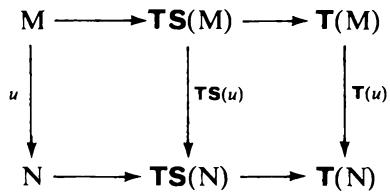
\includegraphics[keepaspectratio]{images/part001_53632150.jpg}}

is commutative, where the horizontal arrows denote canonical injections.

If M is a direct factor of N and \(i: M \rightarrow N\) is the canonical injection, then \(\mathbf{TS}(i)\) is an injective homomorphism of \(\mathbf{TS}(\mathbf{M})\) onto a direct factor R of \(\mathbf{TS}(\mathbf{N})\) , by which we normally identify \(\mathbf{TS}(\mathbf{M})\) and R. That is proved as for the tensor algebra (III, p.~487).

Suppose that M is a direct sum of a family \((\mathbf{M}_{\lambda})_{\lambda \in L}\) of submodules. The canonical injections \(\mathbf{TS}(\mathbf{M}_{\lambda}) \to \mathbf{TS}(\mathbf{M})\) define a unital homomorphism h of graded algebras, called canonical:

\[
\underset {\lambda \in L} {\otimes} \mathbf {T S} \left(\mathrm{M} _ {\lambda}\right)\rightarrow \mathbf {T S} (\mathrm{M}).
\]

Let \(\lambda_1, \lambda_2, \ldots, \lambda_n\) be pairwise distinct elements of \(L\) and let \(x_1 \in M_{\lambda_1}, \ldots, x_n \in M_{\lambda_n}\) . By Prop. 3, (ii) of IV, p.~45 we have

\[
h \left(\sum_ {p _ {1} + \dots + p _ {n} = p} \gamma_ {p _ {1}} (x _ {1}) \otimes \dots \otimes \gamma_ {p _ {n}} (x _ {n})\right) = \gamma_ {p} (x _ {1} + \dots + x _ {n}).\tag{8}
\]

Let N be an A-module which is a direct sum of a family \((\mathbf{N}_{\lambda})_{\lambda \in L}\) of submodules. For every \(\lambda \in L\) let \(u_{\lambda}\) be a homomorphism of \(M_{\lambda}\) into \(N_{\lambda}\) . Let u be the homomorphism of M into N defined by the \(u_{\lambda}\) . Then the diagram

\[
\begin{array}{c} \otimes \mathsf {T S} (\mathrm{M} _ {\lambda}) \xrightarrow {h} \mathsf {T S} (\mathrm{M}) \\ \otimes \mathsf {T S} (u _ {\lambda}) \Bigg | _ {\downarrow} \qquad \qquad \qquad \qquad \qquad \qquad \qquad \qquad \qquad \qquad \qquad \qquad \qquad \qquad \qquad \qquad \qquad \qquad \qquad \qquad \qquad \qquad \qquad \qquad \qquad \qquad \qquad \qquad \qquad \qquad \qquad \qquad \qquad \qquad \\ \otimes \mathsf {T S} (\mathrm{N} _ {\lambda}) \xrightarrow {h ^ {\prime}} \mathsf {T S} (\mathrm{N}) \end{array}
\]

commutes, where h and \(h'\) are canonical homomorphisms. For if \(z \in TS(M_{\lambda})\) and if \(i_{\lambda}\) (resp. \(j_{\lambda}\) ) denotes the canonical injection of \(M_{\lambda}\) into M (resp. \(N_{\lambda}\) into N), then we have

\[
\begin{array}{r l} \mathbf {T S} (u) (h (z)) & = \mathbf {T S} (u) \circ \mathbf {T S} (i _ {\lambda}) (z) = \mathbf {T S} (u \circ i _ {\lambda}) (z) = \\ & = \mathbf {T S} (j _ {\lambda} \circ u _ {\lambda}) (z) = \mathbf {T S} (j _ {\lambda}) \circ \mathbf {T S} (u _ {\lambda}) (z) = h ^ {\prime} (\mathbf {T S} (u _ {\lambda}) (z)). \end{array}
\]

PROPOSITION 6. --- Let M be an A-module which is the direct sum of a family \((\mathbf{M}_{\lambda})_{\lambda \in L}\) of submodules. If each \(M_{\lambda}\) is a free module, then the canonical homomorphism of \(\otimes \mathbf{TS}(\mathbf{M}_{\lambda})\) into \(\mathbf{TS}(\mathbf{M})\) is an isomorphism.

Let \((e_{i,\lambda})_{i\in I_{\lambda}}\) be a basis of \(\mathbf{M}_{\lambda}\) . For \(\nu \in \mathbf{N}^{(I_{\lambda})}\) put \(e_{\nu ,\lambda} = \prod_{i\in I_{\lambda}}\gamma_{\nu (i)}(e_{i,\lambda})\) . The \(e_{\nu ,\lambda}\) for \(\nu \in \mathbf{N}^{(I_{\lambda})}\) form a basis of \(\mathbf{TS}(\mathbf{M}_{\lambda})\) (IV, p.~47, Prop. 4 (i)) and \(e_{0,\lambda}\) is the unit-element of \(\mathbf{TS}(\mathbf{M}_{\lambda})\) . Therefore the elements

\[
\bigotimes_ {\lambda \in L} e _ {\nu_ {\lambda}, \lambda}\tag{9}
\]

where \(\nu_{\lambda} \in \mathbf{N}^{(I_{\lambda})}\) and \(\nu_{\lambda} = 0\) except for a finite number of indices, form a basis of \(\otimes_{\lambda} \mathbf{TS}(M_{\lambda})\) . The image of the element (9) under the canonical homomorphism of the proposition is \(\prod_{\lambda \in L} e_{\nu_{\lambda,\lambda}}\) . If we denote by \((e_i)_{i \in I}\) the disjoint union of the families \((e_{i,\lambda})_{i \in I_{\lambda}}\) , then the above elements are precisely \(\prod_{i \in I} \gamma_{\nu(i)}(e_i)\) , where \(\nu \in \mathbf{N}^{(I)}\) , and so they constitute a basis of \(\mathbf{TS}(M)\) . This proves the proposition.

Under the conditions of Prop. 6, the inverse isomorphism \(\mathbf{TS}(\mathbf{M}) \to \otimes_{\lambda} \mathbf{TS}(\mathbf{M}_{\lambda})\) is also called canonical. Frequently \(\mathbf{TS}(\mathbf{M})\) is identified with

\(\otimes_{\lambda} \mathbf{TS}(M_{\lambda})\) by means of this isomorphism. It should be noted that if \(z \in \mathbf{TS}(M_{\lambda})\)

\pandocbounded{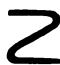
\includegraphics[keepaspectratio]{images/part001_3a9079a2.jpg}}

and \(z' \in \mathbf{TS}(M_{\mu})\) with \(\lambda \neq \mu\) , then the element of TS(M) which we are thus led to denote by \(z \otimes z'\) is not the tensor product of z and \(z'\) in T(M) but the symmetric product of z and \(z'\) .

PROPOSITION 7. --- Let M be an A-module, u the mapping \((x, y) \mapsto x + y\) of \(M \oplus M\) into M and f the composite mapping

\[
\mathbf {T S} (\mathrm{M}) \otimes \mathbf {T S} (\mathrm{M}) \xrightarrow {h} \mathbf {T S} (\mathrm{M} \oplus \mathrm{M}) \xrightarrow {\mathbf {T S} (u)} \mathbf {T S} (\mathrm{M})
\]

where \(h\) is the canonical homomorphism. If \(z, z' \in \mathbf{TS}(\mathbf{M})\) , then \(f(z \otimes z') = zz'\) .

For let \(i\) be the mapping \(x \mapsto (x, 0)\) of M into M ⊕ M. We have \(u \circ i = \mathrm{Id}_{\mathbf{M}}\) , hence \(\mathbf{TS}(u) \circ \mathbf{TS}(i) = \mathrm{Id}_{\mathbf{TS}(\mathbf{M})}\) ; therefore

\[
f (z \otimes 1) = \mathbf {T S} (u) (h (z \otimes 1)) = \mathbf {T S} (u) (\mathbf {T S} (i) (z)) = z.
\]

Likewise \(f(1 \otimes z') = z'\) , whence \(f(z \otimes z') = f(z \otimes 1)\) \(f(1 \otimes z') = zz'\) .

\subsection{Coproduct for symmetric tensors}

Let M be a free A-module, and \(\Delta_{M} = \Delta\) the diagonal homomorphism \(x \mapsto (x, x)\) of M into \(M \oplus M\) . Let \(c_{M} = c\) be the unital homomorphism of graded A-algebras composed of the homomorphisms:

\[
\mathbf {T S} (\mathrm{M}) \xrightarrow {\mathbf {T S} (\Delta)} \mathbf {T S} (\mathrm{M} \oplus \mathrm{M}) \xrightarrow {\sigma} \mathbf {T S} (\mathrm{M}) \otimes \mathbf {T S} (\mathrm{M})
\]

where \(\sigma\) is the canonical isomorphism. Equipped with \(c\) , \(\mathbf{TS}(\mathbf{M})\) is a graded A-cogebra.

For all \(x \in \mathbf{M}\) and each integer \(p \geqslant 0\) we have \(\mathbf{TS}(\Delta) (\gamma_p(x)) = \gamma_p((x, x))\) , hence by (8),

\[
c \left(\gamma_ {p} (x)\right) = \sum_ {r + s = p} \gamma_ {r} (x) \otimes \gamma_ {s} (x).\tag{10}
\]

In particular

\[
c (x) = x \otimes 1 + 1 \otimes x.\tag{11}
\]

Let \((x_{i})_{i\in I}\) be a family of elements of \(\mathbf{M}\) , and for \(\nu \in \mathbf{N}^{(I)}\) put \(x_{\nu} = \prod_{i\in I}\gamma_{\nu_i}(x_i)\) . Then

\[
c \left(x _ {\nu}\right) = \sum_ {\rho + \sigma = \nu} x _ {\rho} \otimes x _ {\sigma}.\tag{12}
\]

This follows from (10) because \(c\) is an algebra homomorphism.

PROPOSITION 8. --- Let M be a free A-module, then with its algebra and cogebra structures, TS(M) is a graded commutative and cocommutative bigebra. The counit is the A-linear mapping \(\varepsilon: \mathbf{TS}(\mathbf{M}) \to \mathbf{TS}^0(\mathbf{M}) = \mathbf{A}\) which is zero on \(\mathbf{TS}^p(\mathbf{M})\) for \(p > 0\) and such that \(\varepsilon(1) = 1\) .

We know that the A-algebra TS(M) is associative, commutative and unital. On the other hand, the coproduct is by construction a homomorphism of graded algebras; now the fact that the cogebra TS(M) is coassociative and cocommutative follows by an easy calculation from the Formula (10). The mapping \(\varepsilon\) of TS(M) into A is a homomorphism of graded algebras such that \(\varepsilon(1)=1\) . Finally for every \(x\in M\) we have \(\varepsilon(\gamma_{p}(x))=0\) if p\textgreater0, \(\varepsilon(\gamma_{0}(x))=1\) ; if we bear in mind (10), this shows that \((\varepsilon\otimes1)\circ c=(1\otimes\varepsilon)\circ c=\mathrm{Id}_{\mathbf{TS}(\mathbf{M})}\) ; thus \(\varepsilon\) is the counit of TS(M).

PROPOSITION 9. --- Let M and N be free A-modules and u an A-homomorphism of M into N; then TS(u) is a bigebra homomorphism.

For we have \(\Delta_{\mathbf{N}} \circ u = (u, u) \circ \Delta_{\mathbf{M}}\) , hence the diagram

\[
\begin{array}{c} \mathsf {T S (M)} \xrightarrow {\mathsf {T S} (\Delta_ {M})} \mathsf {T S (M \oplus M)} \xrightarrow {\sigma} \mathsf {T S (M)} \otimes \mathsf {T S (M)} \\ \mathsf {T S (u)} \Bigg | _ {\mathsf {T S (u)}} \\ \mathsf {T S (N)} \xrightarrow {\mathsf {T S} (\Delta_ {N})} \mathsf {T S (N \oplus N)} \xrightarrow {\tau} \mathsf {T S (N)} \otimes \mathsf {T S (N)}, \end{array}
\]

where \(\sigma\) and \(\tau\) are canonical isomorphisms, is commutative (IV, p.~49). Thus \(c_{\mathrm{N}} \circ \mathbf{T}\mathbf{S}(u) = (\mathbf{T}\mathbf{S}(u) \otimes \mathbf{T}\mathbf{S}(u)) \circ c_{\mathrm{M}}\) .

PROPOSITION 10. --- Let M be a free A-module, then the primitive elements (III, p.~602) of the bigebra TS(M) are the elements of M.

Let \((e_i)_{i\in I}\) be a basis of \(\mathbf{M}\) , and for \(\nu \in \mathbf{N}^{(I)}\) put \(e_{\nu} = \prod_{i\in I}\gamma_{\nu_i}(e_i)\) . Let

\(z = \sum_{\nu \in \mathbf{N}^{(I)}} \lambda_{\nu} e_{\nu}\) be an element of \(\mathbf{T}\mathbf{S}(\mathbf{M})\) , then by (12) we have

\[
c (z) = \sum_ {\nu} \lambda_ {\nu} \sum_ {\rho , \sigma \in \mathbf {N} ^ {(I)}, \rho + \sigma = \nu} e _ {\rho} \otimes e _ {\sigma} = \sum_ {\rho , \sigma} \lambda_ {\rho + \sigma} e _ {\rho} \otimes e _ {\sigma}
\]

hence

\[
c (z) - 1 \otimes z - z \otimes 1 = \sum_ {\rho \neq 0, \sigma \neq 0} \lambda_ {\rho + \sigma} e _ {\rho} \otimes e _ {\sigma} - \lambda_ {0} e _ {0} \otimes e _ {0}.
\]

and so

\[
\begin{array}{r l} z \text {   primitive   } & \Leftrightarrow \lambda_ {\rho + \sigma} = 0 \text {   when   } \rho \neq 0 \text {   and   } \sigma \neq 0 \text {   and   } \lambda_ {0} = 0 \\ & \Leftrightarrow \lambda_ {\nu} = 0 \text {   when   } | \nu | \neq 1 \\ & \Leftrightarrow z \in M. \end{array}
\]

\subsection{Relations between TS(M) and S(M)}

The canonical injection of M in TS(M) extends in a unique fashion to an algebra homomorphism of T(M) into TS(M) (III, p.~485, Prop. 1). By Prop. 2, (ii) of IV, p.~43, this homomorphism is the operator s of symmetrization. Since the algebra TS(M) is commutative there exists (III, p.~497) one and only one algebra homomorphism \(\varphi_{M}\) , called canonical, of the algebra S(M) into the algebra TS(M) such that the diagram

\pandocbounded{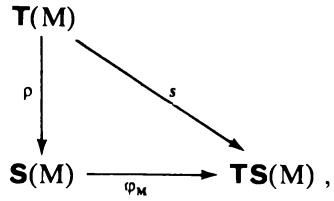
\includegraphics[keepaspectratio]{images/part001_42062a6f.jpg}}

where \(\rho\) denotes the canonical homomorphism of \(\mathbf{T}(\mathbf{M})\) onto \(\mathbf{S}(\mathbf{M})\) , is commutative. We have \(\varphi_{\mathbf{M}}(\mathbf{S}^{p}(\mathbf{M})) \subset \mathbf{T}\mathbf{S}^{p}(\mathbf{M})\) for all \(p \in N\) .

On the other hand, by composing the canonical injection i of TS(M) into T(M) with the canonical homomorphism \(\rho\) of T(M) onto S(M) we obtain a homomorphism \(\psi_{M}\) of graded A-modules, called canonical. The diagram

\pandocbounded{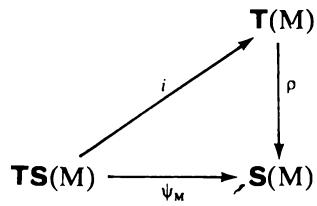
\includegraphics[keepaspectratio]{images/part001_38781a0a.jpg}}

is commutative.

If \(u: \mathbf{M} \to \mathbf{N}\) is a homomorphism of A-modules, then the diagram

\begin{enumerate}
\def\labelenumi{(\arabic{enumi})}
\setcounter{enumi}{12}
\tightlist
\item
\end{enumerate}

\pandocbounded{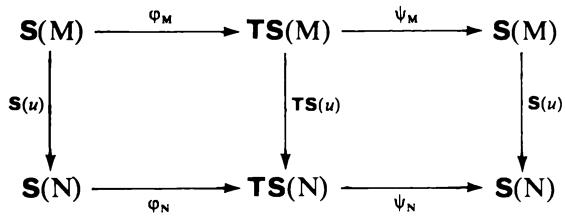
\includegraphics[keepaspectratio]{images/part001_026b2058.jpg}}

is commutative, as is easily verified.

If M is the direct sum of the modules \(M_{\lambda}\) , the diagram

\begin{enumerate}
\def\labelenumi{(\arabic{enumi})}
\setcounter{enumi}{13}
\tightlist
\item
\end{enumerate}

\pandocbounded{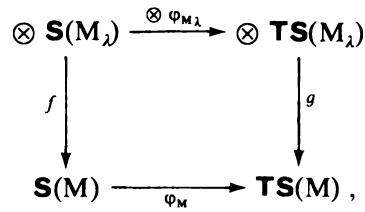
\includegraphics[keepaspectratio]{images/part001_9b5b14d2.jpg}}

where \(f\) and \(g\) are the canonical homomorphisms, is commutative. For \(g \circ \bigotimes_{\lambda} \varphi_{M_{\lambda}}\) and \(\varphi_{M} \circ f\) are algebra homomorphisms which coincide on \(M_{\lambda}\) for every \(\lambda\).

PROPOSITION 11. --- If M is free, then \(\varphi_{\mathbf{M}}\) is a morphism of graded bigebras.

Using the commutativity of the diagrams (13) and (14), we obtain the commutative diagram

\[
\begin{array}{l} \mathbf {S} (\mathrm{M}) \xrightarrow {\mathbf {S} (\Delta)} \mathbf {S} (\mathrm{M} \oplus \mathrm{M}) \xrightarrow {h} \mathbf {S} (\mathrm{M}) \otimes \mathbf {S} (\mathrm{M}) \\ \varphi_ {\mathrm{M}} \Bigg | _ {\downarrow} \quad \Bigg | _ {\varphi_ {\mathrm{M}} \oplus \mathrm{M}} \quad \Bigg | _ {\varphi_ {\mathrm{M}} \otimes \varphi_ {\mathrm{M}}} \\ \mathbf {T S} (\mathrm{M}) \xrightarrow [ \mathsf {T S} (\Delta) ]{} \mathbf {T S} (\mathrm{M} \oplus \mathrm{M}) \xrightarrow [ k ]{} \mathbf {T S} (\mathrm{M}) \cdot \otimes \mathbf {T S} (\mathrm{M}), \end{array}
\]

where \(\Delta\) is the diagonal homomorphism and h, k are canonical homomorphisms. The proposition follows from this.

PROPOSITION 12. --- (i) If \(u \in \mathbf{S}^n(\mathbf{M})\) , then \(\psi_{\mathbf{M}}(\varphi_{\mathbf{M}}(u)) = n!u\) .

\begin{enumerate}
\def\labelenumi{(\roman{enumi})}
\setcounter{enumi}{1}
\tightlist
\item
  If \(v \in \mathbf{T}\mathbf{S}^n(\mathbf{M})\) then \(\varphi_{\mathbf{M}}(\psi_{\mathbf{M}}(v)) = n!v\) .
\end{enumerate}

Let \(x_{1}, \ldots, x_{n} \in M\) and let u be the product \(x_{1} \ldots x_{n}\) calculated in \(\mathbf{S}(\mathbf{M})\) . Then \(\varphi_{\mathbf{M}}(u)\) is the product \(x_{1} \ldots x_{n}\) calculated in \(\mathbf{T}\mathbf{S}(\mathbf{M})\) , that is

\[
\sum_ {\sigma \in \mathfrak {S} _ {n}} x _ {\sigma (1)} \otimes \dots \otimes x _ {\sigma (n)}.
\]

Hence \(\psi_{\mathbf{M}}(\varphi_{\mathbf{M}}(u))\) equals \(\sum_{\sigma \in \mathfrak{S}_n}x_{\sigma (1)}\ldots x_{\sigma (n)}\) calculated in \(\mathbf{S}(\mathbf{M})\) , that is

\[
n! x _ {1} \dots x _ {n} = n! u.
\]

Let \(v = \sum_{i=1}^{p} x_1^i \otimes x_2^i \otimes \ldots \otimes x_n^i\) be an element of \(\mathbf{TS}^n(\mathbf{M})\) , where the \(x_j^i\) belong

to \(\mathbf{M}\) ; then \(\psi_{\mathbf{M}}(v)\) is equal to \(\sum_{i=1}^{p} x_1^i x_2^i \ldots x_n^i\) calculated in \(\mathbf{S}(\mathbf{M})\) , whence

\[
\varphi_ {\mathrm{M}} \big (\psi_ {\mathrm{M}} (v) \big) = \sum_ {i = 1} ^ {p} \mathbf {s} \big (x _ {1} ^ {i} \otimes x _ {2} ^ {i} \otimes \dots \otimes x _ {n} ^ {i} \big) = s (v) = n! v.
\]

COROLLARY 1. --- If A is a Q-algebra, then the canonical homomorphism of S(M) into TS(M) is an algebra isomorphism. If moreover M is free, then it is an isomorphism of graded bigebras.

COROLLARY 2. --- If A is a Q-algebra then the module \(\mathbf{TS}^n (\mathbf{M})\) is generated by the \(n\) -th powers of elements of \(\mathbf{M}\) in \(\mathbf{TS}(\mathbf{M})\) .

This follows from Cor. 1 and the corresponding property of \(\mathbf{S}(\mathbf{M})\) (III, p.~498).

\subsection{Homogeneous polynomial mappings}

PROPOSITION 13. --- Let M and N be A-modules, q an integer ≥ 0, and f a mapping of M into N. Suppose that M is free, then the following conditions are equivalent:

\begin{enumerate}
\def\labelenumi{(\roman{enumi})}
\item
  There exists a \(q\) -linear mapping \(g\) of \(\mathbf{M}^q\) into \(\mathbf{N}\) such that \(f(x) = g(x, x, \ldots, x)\) for all \(x \in \mathbf{M}\) .
\item
  There exists a linear mapping \(h\) of \(\mathbf{T}\mathbf{S}^q (\mathbf{M})\) into \(\mathbf{N}\) such that \(f(x) = h(\gamma_q(x))\) for all \(x \in \mathbf{M}\) .
\item
  There exists a basis \((e_i)_{i\in I}\) of \(\mathbf{M}\) and a family \((u_{\nu})_{\nu \in \mathbf{N}^{(I)},|\nu| = q}\) of elements of \(\mathbf{N}\) such that
\end{enumerate}

\[
f \left(\sum_ {i \in I} \lambda_ {i} e _ {i}\right) = \sum_ {\nu \in \mathbf {N} ^ {(I)}, | \nu | = q} \lambda^ {\nu} u _ {\nu}\tag{15}
\]

for all \((\lambda_i) \in \mathbf{A}^{(I)}\) .

\begin{enumerate}
\def\labelenumi{(\roman{enumi})}
\setcounter{enumi}{3}
\tightlist
\item
  For each basis \((e_i)_{i\in I}\) of \(\mathbf{M}\) there exists a family \((u_{\nu})_{\nu\in \mathbf{N}^{(I)},|\nu| = q}\) of elements of \(\mathbf{N}\) such that
\end{enumerate}

\[
f \left(\sum_ {i \in I} \lambda_ {i} e _ {i}\right) = \sum_ {\nu \in \mathbf {N} ^ {(I)}, | \nu | = q} \lambda^ {\nu} u _ {\nu}
\]

for all \((\lambda_i) \in \mathbf{A}^{(\mathrm{I})}\) .

\begin{enumerate}
\def\labelenumi{(\roman{enumi})}
\tightlist
\item
  \(\Rightarrow\) (ii): let \(g\) satisfy (i), then there exists a linear mapping \(g'\) of \(\mathbf{T}^q (\mathbf{M})\) into \(\mathbf{N}\) such that \(g(x_{1},x_{2},\ldots ,x_{q}) = g'(x_{1}\otimes x_{2}\otimes \ldots \otimes x_{q})\) for any \(x_{1},\ldots ,x_{q}\in \mathbf{M}\) . Then
\end{enumerate}

\[
f (x) = g (x, x, \dots , x) = g ^ {\prime} (x \otimes x \otimes \dots \otimes x) = g ^ {\prime} (\gamma_ {q} (x));
\]

and on writing \(h = g' \mid \mathbf{TS}^q(\mathbf{M})\) we see that condition (ii) holds.

\begin{enumerate}
\def\labelenumi{(\roman{enumi})}
\setcounter{enumi}{1}
\tightlist
\item
  \(\Rightarrow\) (i) and (iv): let \(h\) satisfy the conditions of (ii). By Prop. 4, (ii) (IV, p.~47) there exists a linear mapping \(g'\) of \(\mathbf{T}^q (\mathbf{M})\) into \(\mathbf{N}\) such that \(h = g'|\mathbf{TS}^q (\mathbf{M})\) . Let \(g\) be the \(q\) -linear mapping of \(\mathbf{M}\) into \(\mathbf{N}\) associated with \(g'\) , then for any \(x\in \mathbf{M}\) we have
\end{enumerate}

\[
f (x) = h \left(\gamma_ {q} (x)\right) = g ^ {\prime} (x \otimes x \otimes \dots \otimes x) = g (x, x, \dots , x),
\]

whence (i). On the other hand, if \((e_i)_{i\in I}\) is a basis of \(\mathbf{M}\) , we have, by formula (6) (IV, p.~46)

\[
f \left(\sum_ {i} \lambda_ {i} e _ {i}\right) = h \left(\gamma_ {q} \left(\sum_ {i} \lambda_ {i} e _ {i}\right)\right) = h \left(\sum_ {| \nu | = q} \lambda^ {\nu} e _ {\nu}\right)
\]

on writing \(e_{\nu} = \prod_{i\in I}\gamma_{\nu_i}(e_i)\) ; we thus have

\[
f \left(\sum_ {i} \lambda_ {i} e _ {i}\right) = \sum_ {| \nu | = q} \lambda^ {\nu} h \left(e _ {\nu}\right).
\]

\begin{enumerate}
\def\labelenumi{(\roman{enumi})}
\setcounter{enumi}{3}
\item
  \(\Rightarrow\) (iii) is clear.
\item
  \(\Rightarrow\) (ii): given \((e_i)\) , \((u_\nu)\) satisfying the conditions of (iii), let us write \(e_\nu = \prod_{i\in I}\gamma_{\nu_i}(e_i)\) and recall that \((e_\nu)_{|\nu| = q}\) is a basis of \(\mathbf{TS}^q (\mathbf{M})\) . Let \(h\) be the homomorphism of \(\mathbf{TS}^q (\mathbf{M})\) into \(\mathbf{N}\) defined by \(h(e_{\nu}) = u_{\nu}\) ; then for each \(x = \sum_{i\in I}\lambda_i e_i\) in \(\mathbf{M}\) we have
\end{enumerate}

\[
f (x) = f \left(\sum_ {i} \lambda_ {i} e _ {i}\right) = \sum_ {| \nu | = q} \lambda^ {\nu} u _ {\nu} = h \left(\sum_ {| \nu | = q} \lambda^ {\nu} e _ {\nu}\right) = h (\gamma_ {q} (x)).
\]

DEFINITION 3. --- Let M and N be A-modules and q an integer \(\geqslant 0\) . Suppose that M is free, and denote by \(\operatorname{Pol}_{\mathbf{A}}^{q}(\mathbf{M}, \mathbf{N})\) or simply \(\operatorname{Pol}^{q}(\mathbf{M}, \mathbf{N})\) the set of mappings of M into N satisfying the conditions of Prop. 13. The elements of \(\operatorname{Pol}^{q}(\mathbf{M}, \mathbf{N})\) are called homogeneous polynomial mappings of degree q of M into N.

Prop. 13 (i) defines a homomorphism of A-modules :

\[
\mathcal {L} _ {q} (\mathrm{M}, \dots , \mathrm{M}; \mathrm{N}) \rightarrow \operatorname{Pol} ^ {q} (\mathrm{M}, \mathrm{N}).
\]

Prop. 13 (ii) defines a homomorphism of A-modules :

\[
\operatorname{Hom} _ {\mathrm{A}} \left(\mathbf {T S} ^ {q} (\mathrm{M}), \mathrm{N}\right)\rightarrow \operatorname{Pol} ^ {q} (\mathrm{M}, \mathrm{N}).
\]

These homomorphisms are called canonical. They are surjective.

Examples. --- 1) The homogeneous polynomial mappings of degree 1 of M into N are the A-linear mappings of M into N.

\begin{enumerate}
\def\labelenumi{\arabic{enumi})}
\setcounter{enumi}{1}
\tightlist
\item
  Let \((\mathbf{N}_i)_{i\in I}\) be a family of A-modules, \(f_{i}\) a mapping of \(\mathbf{M}\) into \(\mathbf{N}_i\) , \(i\in I\) , and \(f:\mathbf{M}\to \prod_{i\in I}\mathbf{N}_i\) the mapping with components \(f_{i}\) . For \(f\) to be a
\end{enumerate}

homogeneous polynomial mapping of degree q it is necessary and sufficient that each \(f_{i}\) be a homogeneous polynomial mapping of degree q.

\begin{enumerate}
\def\labelenumi{\arabic{enumi})}
\setcounter{enumi}{2}
\item
  Let \((\mathbf{M}_j)_{j\in J}\) be a finite family of free A-modules and \(u:\prod_{j\in J}\mathbf{M}_j\to \mathbf{N}\) a multilinear mapping; then \(u\) is polynomial of degree Card(J).
\item
  Let \((\mathbf{X}_i)_{i\in I}\) be a family of indeterminates, N an A-module and \(u\in \mathbf{N}[(\mathbf{X}_i)_{i\in I}]\) a homogeneous polynomial of degree \(q\) . The mapping \((x_{i})_{i\in I}\mapsto u((x_{i})_{i\in I})\) of \(\mathbf{A}^{(I)}\) into N is a homogeneous polynomial mapping of degree \(q\) : this is seen at once by condition (iii) of Prop. 13. If I is finite, every homogeneous polynomial mapping of degree \(q\) of \(\mathbf{A}^{(I)} = \mathbf{A}^{\mathrm{I}}\) into N is of that form.
\item
  The mapping \((x_{i})_{i\in\mathbf{N}}\mapsto x_{0}^{2}+x_{1}^{2}+\cdots+x_{n}^{2}+\cdots\) of \(\mathbf{A}^{(N)}\) into A is a homogeneous polynomial mapping of degree 2. If A=Z/2Z, it coincides with the linear mapping \((x_{i})_{i\in I}\mapsto x_{0}+x_{1}+\cdots+x_{n}+\cdots\)
\item
  Let \(f \in \operatorname{Pol}_{\mathbf{A}}^{q}(\mathbf{M}, \mathbf{N})\) , let \(\mathbf{B}\) be a commutative ring, \(\rho\) a homomorphism of \(\mathbf{B}\) into \(\mathbf{A}\) and \(\mathbf{M}'\) and \(\mathbf{N}'\) the B-modules derived from \(\mathbf{M}\) and \(\mathbf{N}\) by means of \(\rho\) . Assume that \(\mathbf{M}'\) is free; then \(f \in \operatorname{Pol}_{\mathbf{B}}^{q}(\mathbf{M}', \mathbf{N}')\) : this follows at once from condition (i) of Prop. 13.
\end{enumerate}

PROPOSITION 14. --- Let M, N, P be A-modules, q and r integers ≥ 0, and assume that M and N are free. If \(f \in \text{Pol}^{q}(M, N)\) , \(f' \in \text{Pol}^{r}(N, P)\) , then \(f' \circ f \in \text{Pol}^{qr}(M, P)\) .

There exists a q-linear mapping g of \(M^{q}\) into N and an r-linear mapping \(g'\) of \(N^{r}\) into P such that

\[
\begin{array}{l l} f (x) = g (x, x, \dots , x) & \text { for   all } x \in \mathbf {M}, \\ f ^ {\prime} (y) = g ^ {\prime} (y, y, \dots , y) & \text { for   all } y \in \mathbf {N}. \end{array}
\]

Hence for every \(x \in \mathbf{M}\) we have

\[
f ^ {\prime} (f (x)) = g ^ {\prime} (f (x), f (x), \dots , f (x)) = g ^ {\prime} (g (x, x, \dots , x), \dots , g (x, x, \dots , x))
\]

and the mapping \((x_{1},\ldots ,x_{qr})\mapsto g^{\prime}\big(g(x_{1},\dots,x_{q}),\dots,g(x_{q(r - 1) + 1},\dots,x_{qr})\big)\) of \(\mathbf{M}^{qr}\) into \(\mathbf{P}\) is \(qr\) -linear.

PROPOSITION 15. --- Let M be a free A-module, N an A-module and q an integer \(\geqslant0\) . We suppose that the mapping \(y\mapsto q!y\) is an automorphism of N. Let \(f\in\mathrm{Pol}^{q}(\mathbf{M},\mathbf{N})\) , then there exists one and only one symmetric q-linear mapping h of \(M^{q}\) into N such that \(f(x)=h(x,x,\ldots,x)\) for all \(x\in M\) . For any \(x_{1},\ldots,x_{q}\in M\) we have

\[
h \left(x _ {1}, x _ {2}, \dots , x _ {q}\right) = \frac {(- 1) ^ {q}}{q !} \sum_ {\mathrm{H} \subset \{1, 2, \dots , q \}} (- 1) ^ {\text { Card   H }} f \left(\sum_ {i \in \mathrm{H}} x _ {i}\right).\tag{16}
\]

\begin{enumerate}
\def\labelenumi{\alph{enumi})}
\tightlist
\item
  There exists a \(q\) -linear mapping \(g\) of \(\mathbf{M}^q\) into \(\mathbf{N}\) such that \(f(x) = g(x, x, \ldots, x)\) for all \(x \in \mathbf{M}\) . Let us define a \(q\) -linear mapping \(h\) of \(\mathbf{M}\) into \(\mathbf{N}\) by
\end{enumerate}

\[
h \left(x _ {1}, x _ {2}, \dots , x _ {q}\right) = \frac {1}{q !} \sum_ {\sigma \in \mathfrak {S} _ {q}} g \left(x _ {\sigma (1)}, x _ {\sigma (2)}, \dots , x _ {\sigma (q)}\right).
\]

Then \(h\) is symmetric and \(f(x) = h(x, x, \ldots, x)\) for all \(x \in \mathbf{M}\) .

\begin{enumerate}
\def\labelenumi{\alph{enumi})}
\setcounter{enumi}{1}
\tightlist
\item
  Let \(h\) be a symmetric \(q\) -linear mapping of \(\mathbf{M}^q\) into \(\mathbf{N}\) such that \(f(x) = g(x, x, \ldots, x)\) . Let \(l\) be the linear mapping of \(\mathbf{T}^q(\mathbf{M})\) into \(\mathbf{N}\) such that \(h(x_1, \ldots, x_q) = l(x_1 \otimes \ldots \otimes x_q)\) for any \(x_1, \ldots, x_q \in \mathbf{M}\) . We have
\end{enumerate}

\[
\begin{array}{l} (- 1) ^ {q} q! h (x _ {1}, \dots , x _ {q}) = (- 1) ^ {q} \sum_ {\sigma \in \mathfrak {S} _ {q}} h (x _ {\sigma (1)}, \dots , x _ {\sigma (q)}) = \\ = (- 1) ^ {q} l (\mathbf {s} (x _ {1} \otimes \dots \otimes x _ {q})) = \sum_ {\mathrm{H} \subset \{1, \dots , q \}} (- 1) ^ {\text {Card H}} l \left(\gamma_ {q} \left(\sum_ {i \in \mathrm{H}} x _ {i}\right)\right) \end{array}
\]

by Prop. 3, (v) (IV, p.~45). Now

\[
l \left(\gamma_ {q} \left(\sum_ {i \in H} x _ {i}\right)\right) = h \left(\sum_ {i \in H} x _ {i}, \dots , \sum_ {i \in H} x _ {i}\right) = f \left(\sum_ {i \in H} x _ {i}\right)
\]

and this proves formula (16) and the uniqueness of h.

PROPOSITION 16. --- Let M be a free A-module, N an A-module, q a positive integer and u the canonical homomorphism of Hom(TS \(^{q}\) (M), N) into Pol \(^{q}\) (M, N).

\begin{enumerate}
\def\labelenumi{(\roman{enumi})}
\item
  If \(\mathbf{A}\) is an infinite integral domain and \(\mathbf{N}\) is torsion-free, then \(u\) is an isomorphism.
\item
  If the mapping \(y \mapsto q!y\) in \(\mathbf{N}\) is injective, \(u\) is an isomorphism.
\end{enumerate}

In the two cases of the proposition we have to prove that \(u\) is injective, that is, every linear mapping \(f\) of \(\mathbf{TS}^q(\mathbf{M})\) into \(\mathbf{N}\) which is zero on \(\gamma_q(\mathbf{M})\) , vanishes.

Assume A to be an infinite integral domain and N torsion-free. For every \(z \in \mathbf{TS}^{q}(\mathbf{M})\) there exists \(\alpha \in A - \{0\}\) such that \(\alpha z\) is an A-linear combination of elements of \(\gamma_{q}(\mathbf{M})\) (IV, p.~47, Prop. 5). Hence \(\alpha f(z) = f(\alpha z) = 0\) , and so \(f(z) = 0\) .

Suppose next that the mapping \(y \mapsto q!y\) in \(\mathbf{N}\) is injective, then by IV, p.~45, Prop. 3, (v), \(f\) vanishes on \(\mathbf{s} \cdot \mathbf{T}^q(\mathbf{M})\) . Hence if \(z \in \mathbf{T}\mathbf{S}^q(\mathbf{M})\) , we have \(q!f(z) = f(\mathbf{s}z) = 0\) , and so \(f(z) = 0\) .

COROLLARY. --- Let M be a free A-module, N an A-module, q a positive integer, \(h \in \operatorname{Pol}^{q}(M, N)\) and \((e_{i})_{i \in I}\) a basis of M. In the two cases of Prop. 16 there exists a unique family \((u_{\nu})_{\nu \in \mathbf{N}^{(I)}, |\nu| = q}\) of elements of N such that \(h\left(\sum_{i \in I} \lambda_{i} e_{i}\right) = \sum_{|\nu| = q} \lambda^{\nu} u_{\nu}\) for all \((\lambda_{i}) \in \mathbf{A}^{(I)}\) .

\subsection{Polynomial mappings}

DEFINITION 4. --- Let M and N be A-modules and assume that M is free. Let \(\operatorname{Map}(M, N)\) be the A-module of all mappings of M into N. The submodule \(\sum_{q > 0} \operatorname{Pol}_{A}^{q}(M, N)\) of \(\operatorname{Map}(M, N)\) is denoted by \(\operatorname{Pol}_{A}(M, N)\) or simply \(\operatorname{Pol}(M, N)\) ;

its elements are called polynomial mappings of M into N.

Let \((e_{i})_{i\in I}\) be a basis of M and suppose that I is finite; by Prop. 13 (IV, p.~54) a mapping f of M into N is polynomial if and only if there exists a polynomial F in the indeterminates \(X_{i}\) with coefficients in N such that

\[
f \left(\sum_ {i \in I} x _ {i} e _ {i}\right) = F (\mathbf {x})
\]

for every family \(\mathbf{x} = (x_i)_{i\in I}\) in \(\mathbf{A}^{(I)}\) . This property is independent of the basis chosen for \(\mathbf{M}\) and it justifies the terminology « polynomial mapping ».

PROPOSITION 17. --- Let M be a free A-module and B an associative, commutative and unital A-algebra. Then \(\operatorname{Pol}_{\mathbf{A}}(\mathbf{M}, \mathbf{B})\) is a sub-B-algebra of the algebra \(\operatorname{Map}(\mathbf{M}, \mathbf{B})\) .

This follows from Def. 4 and Prop. 13, (iv) (IV, p.~54).

PROPOSITION 18. --- Let M, N, P be A-modules, and assume that M and N are free. If \(f \in \operatorname{Pol}(M, N)\) , \(g \in \operatorname{Pol}(N, P)\) , then \(g \circ f \in \operatorname{Pol}(M, P)\) .

We can reduce at once to the case where there exists an integer q such that \(g \in \text{Pol}^{q}(N, P)\) ; then there exists a q-linear mapping h of \(N^{q}\) into P such that \(g(y) = h(y, y, \ldots, y)\) for all \(y \in N\) . Writing f as a sum of homogeneous polynomial mappings we are thus reduced to proving that the mapping

\[
x \mapsto h (f _ {1} (x), f _ {2} (x), \dots , f _ {q} (x))
\]

of M into P, where \(f_{i} \in \operatorname{Pol}^{q_{i}}(\mathbf{M}, \mathbf{N})\) , is polynomial. For \(i = 1, \ldots, q\) there exists a \(q_{i}\) -linear mapping \(l_{i}\) of \(M^{q_{i}}\) into N such that \(f_{i}(x) = l_{i}(x, x, \ldots, x)\) for all \(x \in M\) . Hence

\[
h \left(f _ {1} (x), f _ {2} (x), \dots , f _ {q} (x)\right) = h \left(l _ {1} (x, \dots , x), \dots , l _ {q} (x, \dots , x)\right),
\]

from which our assertion follows.

Lemma 2. --- Let N be an A-module, n an integer ≥0 and

\[
f = m _ {0} + m _ {1} \mathrm{X} + \dots + m _ {n} \mathrm{X} ^ {n} \in \mathrm{N} [ \mathrm{X} ].
\]

Suppose that there exist \(\alpha_{0}, \alpha_{1}, \ldots, \alpha_{n} \in A\) such that \(f(\alpha_{0}) = \cdots = f(\alpha_{n}) = 0\) , and such that for \(i \neq j\) the homothety of ratio \(\alpha_{i} - \alpha_{j}\) in N is injective, then f = 0.

(This lemma generalizes the Cor. of IV, p.~16.)

The lemma clearly holds for \(n = 0\) ; we shall prove it by induction on \(n\) . We have

\[
f (\mathbf {X}) = f (\mathbf {X}) - f \left(\alpha_ {0}\right) = \sum_ {i = 1} ^ {n} m _ {i} \left(\mathbf {X} ^ {i} - \alpha_ {0} ^ {i}\right) = \left(\mathbf {X} - \alpha_ {0}\right) g (\mathbf {X})
\]

where g is an element of N{[}X{]} of the form \(m_{0}^{\prime} + m_{1}^{\prime} X + \cdots + m_{n-1}^{\prime} X^{n-1}\) . The hypotheses of the lemma imply that \(g(\alpha_{1}) = \cdots = g(\alpha_{n}) = 0\) , hence g = 0 by the induction hypothesis, and so f = 0.

PROPOSITION 19. --- Let M be a free A-module, N an A-module, G an infinite additive subgroup of A, and suppose that the homotheties of N defined by the nonzero elements of G are injective. Then \(\operatorname{Pol}(M,N)\) is the direct sum of the \(\operatorname{Pol}^{q}(M,N)\) .

Let \(f_{0}, f_{1}, \ldots, f_{n}\) be such that \(f_{i} \in \operatorname{Pol}^{i}(\mathbf{M}, \mathbf{N})\) and suppose that we have the relation \(f_{0} + \cdots + f_{n} = 0\) . Let \(x \in \mathbf{M}\) , then for all \(\lambda \in G\) we have

\[
0 = \sum_ {i = 0} ^ {n} f _ {i} (\lambda x) = \sum_ {i = 0} ^ {n} \lambda^ {i} f _ {i} (x).
\]

By Lemma 2, applied to the polynomial \(\sum_{i=0}^{n} f_i(x) X^i\) we have

\[
f _ {0} (x) = \dots = f _ {n} (x) = 0.
\]

COROLLARY. --- Assume that A is an infinite integral domain; let M be a free A-module and N a torsion-free A-module.

\begin{enumerate}
\def\labelenumi{(\roman{enumi})}
\tightlist
\item
  We have \(\operatorname{Pol}(\mathbf{M},\mathbf{N}) = \bigoplus_{q\geqslant 0}\operatorname{Pol}^q (\mathbf{M},\mathbf{N})\) and each \(\operatorname{Pol}^q (\mathbf{M},\mathbf{N})\) may be
\end{enumerate}

identified canonically with \(\operatorname{Hom}(\mathbf{TS}^q(\mathbf{M}),\mathbf{N})\) .

\begin{enumerate}
\def\labelenumi{(\roman{enumi})}
\setcounter{enumi}{1}
\tightlist
\item
  Let \(f \in \operatorname{Pol}(M, N)\) and \((e_i)_{i \in I}\) a basis of \(M\) . There exists one and only one family \((u_\nu)_{\nu \in \mathbb{N}^{(I)}}\) of elements of \(N\) such that \(f\left(\sum_{i \in I} \lambda_i e_i\right) = \sum_{\nu \in \mathbb{N}^{(I)}} \lambda^\nu u_\nu\) for all
\end{enumerate}

\[
\left(\lambda_ {i}\right) \in \mathbf {A} ^ {(I)}
\]

The assertion (i) follows from Prop. 16 and 19, and (ii) follows from (i) and the Cor. of Prop. 16.
